\documentclass[a4paper]{article}
\usepackage[french]{babel}
\usepackage{geometry}
\geometry{a4paper}
\usepackage[utf8]{inputenc}
\usepackage{graphicx}
\graphicspath{ {./data/} }
\usepackage{amsmath}
\usepackage{amssymb}
\usepackage{listings}
\usepackage{xcolor}
\usepackage{cite}
\usepackage{color}
\usepackage{float}
\usepackage{soul}


\definecolor{mGreen}{rgb}{0,0.6,0}
\definecolor{mGray}{rgb}{0.5,0.5,0.5}
\definecolor{mPurple}{rgb}{0.58,0,0.82}
\definecolor{backgroundColour}{rgb}{0.95,0.95,0.95}

\lstdefinestyle{CStyle}{
	backgroundcolor=\color{backgroundColour},   
	commentstyle=\color{mGreen},
	keywordstyle=\color{magenta},
	numberstyle=\tiny\color{mGray},
	stringstyle=\color{mPurple},
	basicstyle=\footnotesize,
	breakatwhitespace=false,         
	breaklines=true,                 
	captionpos=b,                    
	keepspaces=true,                 
	numbers=left,                    
	numbersep=5pt,                  
	showspaces=false,                
	showstringspaces=false,
	showtabs=false,                  
	tabsize=2,
	language=C,
	morekeywords={uint32_t, uint16_t, uint8_t, Tc, Dac, Port, inline,state_t}
}


\title{\textbf{projet} \\ document}

\author{Louison GOUY \and Yiying WEI}

\begin{document}

\maketitle

\vspace{2cm}

\begin{center}
   % \includegraphics[width=12cm]{logo_tp.jpg}
\end{center}

\vspace*{1cm}

\begin{center}
    name
\end{center}

\vspace*{7cm}

\begin{center}

abstract
\end{center}

\newpage
\vspace*{3cm}
\begin{quotation}
	"It's not you can use C to generate good code for hardware. If you think like a comupter writing C actually makes sens."
\end{quotation}
\begin{flushright}
	Linus Torvalds
\end{flushright} 
\newpage


\newpage
\renewcommand{\contentsname}{Table des Matières}
\tableofcontents
\newpage
\renewcommand\listfigurename{Liste des figures}
\listoffigures
\newpage

\section{Glossaire}

\textbf{Requête d'interruption} : (IRQ : interrupt request) Signal matériel indiquant qu'une interruption est requise. \\ ~ \\

\textbf{Polling} : approche d'ordonnancement dans laquelle le logiciel répète un test sur une condition pour déterminer s'il doit exécuter une tache.\cite{ARM_book} \\ ~ \\

Une\textbf{ machine état ou automate fini} est une construction mathématique abstraite, susceptible d'être dans un nombre fini d'\textit{états} , mais étant un moment donné dans un seul état à la fois. Le passage d'un état à un autre ce fait par une \textit{transition}. 

\newpage

\section{Le langage C}
Le langage C est un langage combiné, il a les caractéristiques des langages évolués (boucles itératives etc.) associé à des fonctionnalités des langages assemblés (décalage de bit, adressage indirect généralisé etc.). C'est la combinaison de ces deux caractéristiques qui font la force du langage\cite{Monteil2012}. Sa proximité avec l'assembleur le rendant très efficace, il est ainsi devenu le langage indispensable dans la programmation des applications comme l'automatique, la robotique, les OS ect. Cette même proximité impose peu de contraintes à l'utilisateur sur la structure de son programme. Aussi, il est possible d'écrire des fonctions avec plusieurs points de sorties, ou encore, d'échapper à une boucle avant son terme. Là où certains trouveront une grande souplesse, les critiques le considérerons trop permissif. On notera qu'un certain nombre d'organismes officiels proposent un ensemble de règles visant, tout en conservant son efficacité, à éviter les problèmes liés à une programmation peu soignée. L'Agence National de la Sécurité des Systèmes Informatiques française (ANSSI) propose un rapport complet, \textit{Règles de programmation pour le développement sécurisé de logiciels en langage C}\cite{ANSSI2021}, visant à "favoriser la production de logiciels C plus sécurisés, plus sûrs, d’une plus grande robustesse et portables". Il servira de référence durant ce projet.

\newpage

\section{Programme de base} % touver un meilleur titre

Dans un premier temps un nouveau projet est créé de type "GCC C ASF Board project". Microchip studio génère alors une arborescence de fichiers dont un main.c. Ce dernier est étudié de manière globale puis affinée par étape dans la section suivante.

\subsection{Vue globale}
Cette partie détaille le fonctionnement du programme de base. 


\begin{lstlisting}[style=CStyle]
#include <asf.h>

int main (void)
{
	system_init();
	
	/* Insert application code here, after the board has been initialized. */
	
	/* This skeleton code simply sets the LED to the state of the button. */
	while (1) {
		/* Is button pressed? */
		if (port_pin_get_input_level(BUTTON_0_PIN) == BUTTON_0_ACTIVE) {
			/* Yes, so turn LED on. */
			port_pin_set_output_level(LED_0_PIN, LED_0_ACTIVE);
		} else {
			/* No, so turn LED off. */
			port_pin_set_output_level(LED_0_PIN, !LED_0_ACTIVE);
		}
	\end{lstlisting}
	La première ligne permet d'inclure la  bibliothèque asf et ainsi de profiter du niveau d'abstraction mis à disposition par Microship. La suivante, \texttt{int main ()} bien connue des développeurs C, est le point d'entré du programme. C'est la première fonction exécutée. La ligne 5 \texttt{system\_init();} a été générée automatiquement par le logiciel à la création du projet. C'est elle qui nous offre ce niveau d'abstraction en initialisant les horloges et les entrées/sorties etc. Elle est spécifique à la cible utilisée, dans notre cas la carte Microchip SAMD21 Xplained Pro. La ligne 10 correspond à l'implémentation d'une boucle infinie. Cette dernière permet de lire l'état du bouton (ligne 12) en "continu". La condition suivante d’éclanche le résultat souhaité : allumage ou extinction de la LED0.
	
	\subsection{Affinage}
	
	\paragraph{Include ASF}
	~~\\
	L'Advanced Software Framework (ASF) fournit un riche ensemble de pilotes éprouvés et de modules de code développés par des experts pour réduire le temps de conception. Il simplifie l'utilisation des microcontrôleurs en fournissant une abstraction au matériel. ASF est une bibliothèque de code gratuite et open-source conçue pour être utilisée lors des phases d'évaluation, de prototypage, de conception et de production. Elle sera utilisée tout au long de ce TP et fera l'objet de nombreuses références.
	
	\paragraph{System\_init}
	~~\\
	Au début du \texttt{main} la fonction \texttt{system\_init()} est appelée. Comme son nom l'indique elle a pour but d'initialiser le système. Elle est définie dans le fichier \texttt{system.c} et consiste en un simple appel successif à cinq fonctions de configuration : 	 
	\texttt{system\_clock\_init();}
	\texttt{system\_board\_init();}
	\texttt{\_system\_events\_init();}
	\texttt{\_system\_extint\_init();}
	et  \texttt{\_system\_divas\_init();}.
	Elles jouent chacune un rôle essentiel dans l'initialisation de carte.
	
	\paragraph{Boucle infinie}
	~~\\
	Implémenté à travers un \texttt{tant que VRAI}, cette ligne n'est pas difficile à comprendre mais il peut être intéressant d'en établir le contexte. Le guide des bonnes de pratiques de l'ANSSI\cite{ANSSI2021} indique toutefois que la forme d'une boucle infinie est bien \texttt{while(1)} et non \texttt{for(;;)}\\
	De manière générale, le bouclage répète un jeu d'instruction jusqu'à se qu'une condition particulaire soit atteinte. On définit une boucle infinie dès lors que cette condition n'arrive jamais en raison d'une caractéristique inhérente à la boucle. Dans notre cas la condition de sortie serait VRAI=FAUX. C'est impossible ! \\
	Du point de vue matériel l'utilisation d'une boucle infinie permet de borner le programme compteur (PC) dans un espace mémoire bien définit. Le compilateur devrait l'interpréter par un jump ou jmp. Le mieux est probablement de le vérifier. Un fichier \texttt{loop.c} est créé, volontairement le plus simple possible.
	\begin{lstlisting}[style=CStyle]
		/* file loop.c */
		void main(void){while(1);}
	\end{lstlisting}
	Puis la commande \texttt{gcc -S -fverbose-asm loop.c} est exécutée dans un terminal linux. Un fichier \texttt{loop.s} apparaît. L'option \texttt{-S} indique la génération du code assembleur et \texttt{-fverbose-asm} ajoute des commentaires tel que la ligne C correspondant à l'instruction. On extrait du résultat la partie qui nous intéresse :
	\begin{lstlisting}[language={[x86masm]Assembler}]
		;file loop.s
		.L2:
		# loop.c:2: 	while (1);
		jmp	.L2	#
	\end{lstlisting}
	Le compilateur gcc a bien implémenté la boucle infinie via une instruction jump indiquant un saut du PC. Dans cette exemple, la boucle étant vide, le PC saute au même endroit. Il est intéressant de faire le parallèle avec l'assembleur. Cet exemple reste toutefois approximatif puisque ce n'est pas le jeux d'instruction du CORTEXM0+ qui a été utilisé. Prenons le comme une introduction.
	
	\paragraph{Condition sur E/S}
	~~\\
	Les lignes suivantes implémentées via une structure \texttt{if else} traduisent le comportement souhaité du point de vue utilisateur. A savoir, le maintient en position enfoncé du bouton provoque l'illumination de la LED0. La lecture de son état est permis grâce à la fonction \textbf{port\_pin\_get\_input\_level} retournant un entier de valeur \hl{XX} ou XX. Elle est alors comparé à \texttt{LED\_0\_ACTIVE} définit comme XX. Si la condition est vrai la fonction \texttt{port\_pin\_set\_output\_level} est appelé avec comme paramètre \texttt{LED\_0\_ACTIVE} sinon \texttt{!LED\_0\_ACTIVE}.
	
	
	\newpage
	\section{Programmation d'un timer}
	Cette étape vise à générer un signal carré de période 1ms sur une des sorties timer du microcontrôleur. Il s'agit  de préparer l'implantation de la fonction Horloge. Cette fonction sera donc réalisée par une ressource matérielle du microcontrôleur : un timer.
	\subsection{Fonctionnement d'un timer}
	Le microcontrôleur SAMD21 possède 5 timers/counters allant de TC3 à TC7. Il est possible de les paramétrer en fonction de l’utilisation qu’il en sera fait. Dans notre cas, le timer TC6 est imposé par le sujet du TP.\\
	Chaque timer peut prendre 3 configurations possibles : 8, 16 ou 32 bits\footnote{Le timer 32bits fonctionne en assemblant 2 timers 16 bits en cascade}. Le nombre de registres associés à chacune des configurations est différent. Nous utiliserons le mode 16 bits (65536 valeurs possibles).  \\
	\paragraph{Fonctionnement du TC en mode waveform}
	~~\\
	Les timers/counters (TC) du microcontrôleur SAMD21 proposent un mode de fonctionnement adapté à la production de signaux logiques : le mode {\sl waveform}. La sélection du mode se fait via la configuration de certains registres. L'objectif est de générer un signal rectangulaire de rapport cyclique quelconque. \\
	Il existe 4 modes de fonctionnement pour les compteurs en mode WAVEFORM présenté par la figure ci-dessous. \\
	
	\begin{figure}[H]
		\centering
		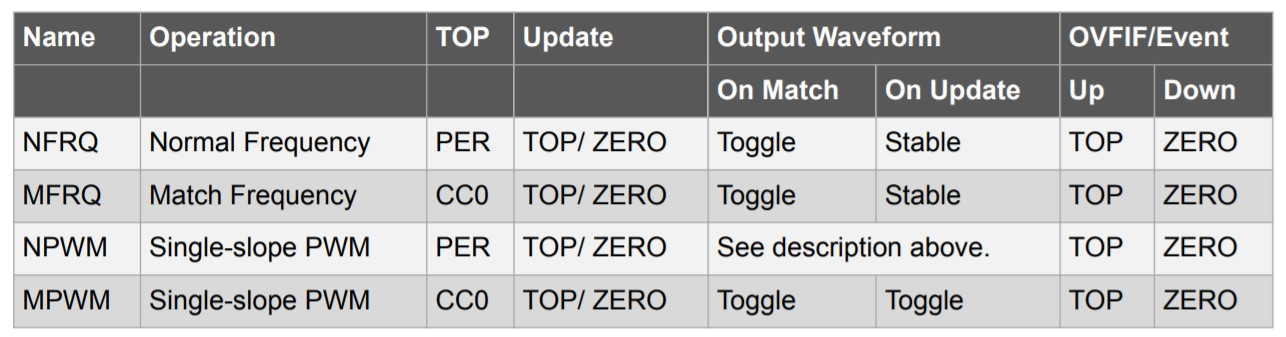
\includegraphics[width=0.9\linewidth]{mode Waveform.jpg}
		\caption{Mode de fonctionnement en WAVEFORM pour les compteurs}
	\end{figure}
	
	Le mode Match Frequency Generation (MFRQ) est le plus adapté à l'application. En effet, la fréquence n'est fixée qu'avec un seul paramètre : CC0. D'après la datasheet du SAMD21, le fonctionnement du mode MFRQ est le suivant. \\
	
	\begin{figure}[H]
		\centering
		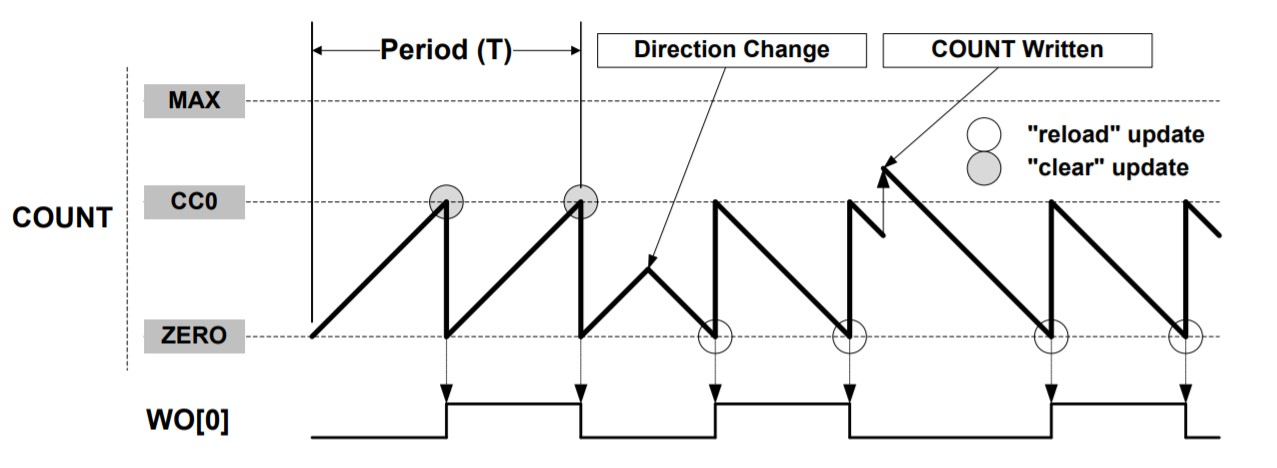
\includegraphics[width=0.85\linewidth]{Match Frequency Operation.jpg}
		\caption{Fonctionnement timer configuré en MFRQ}
	\end{figure}
	La période T du signal est contrôlée par le registre CC0. Le signal de sortie est numérique, sa valeur se trouve dans WO[0]. A chaque fois que le compteur COUNT atteint la valeur du registre CC0.  Le signal de sortie WO[0] est permuté. La valeur MAX correspond à la résolution du compteur : ici 16 bits donc 65536 valeurs possibles. Il faudra être vigilent car la fréquence du compteur vaut deux fois celle du signal de sortie.\\
	
	\paragraph{Calculs pour une fréquence de 1kHz}
	~~\\
	Pour obtenir une fréquence de 1kHz il faut déterminer la valeur de CC0 comme expliqué précédemment. Pour faire cela il est primordial de bien comprendre son fonctionnement et les registres impliqués dans la configuration. La figure ci-dessous donne la fréquence de comptage. \\
	
	\begin{figure}[H]
		\centering
		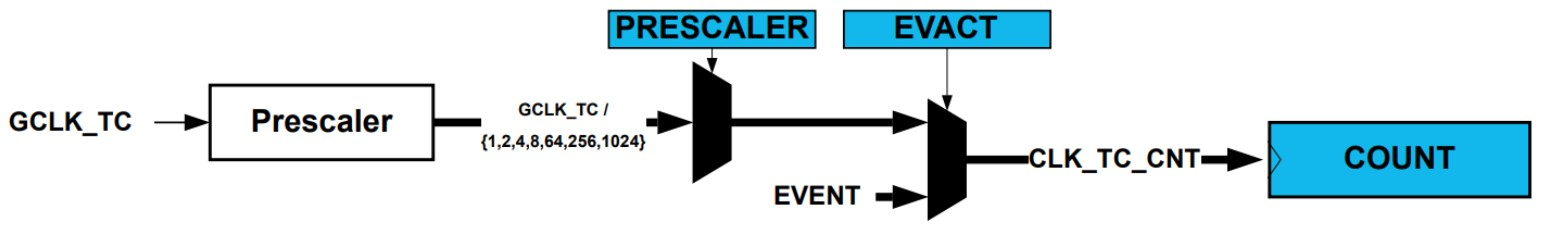
\includegraphics[width=12cm]{prescaler.jpg}
		\caption{Représentation digramme bloc TC}
	\end{figure}
	
	L'horloge count est fournie à partir de l’horloge GCLK\_TC (Generic clock for TC). Elle est l'horloge de référence pour les TC. Elle a une fréquence de 8MHz. Cette horloge peut être divisée en y appliquant un prescaler afin d’obtenir CLK\_TC\_CNT. N est une pré division de l’horloge du timer. Dans notre cas, le prescaler n’est pas appliqué et prendra la valeur N = 1. L'équation ci-dessous présente la fréquence à laquelle sera effectué le comptage. \\
	\begin{equation}
		T_{GCLK\_TC} = N*T_{CLK\_TC\_CNT} = T_{CLK\_TC\_CNT}
	\end{equation}
	On sait que $f_{GCLK\_TC}$ est égale à 8 MHz. Pour une fréquence $f_{WO[0]}$ de 1kHz, on obtient :
	\begin{equation}
		f_{WO[0]} = \frac{f_{CLK\_TC\_CNT}}{2*(CC0+1)}
		\quad \Rightarrow \quad 
		CC0 = \frac{f_{GCLK\_TC}}{2*f_{WO[0]}} - 1 = 3999
	\end{equation}
	La valeur chargée dans le registre CC0 sera donc 3999.
	
	\subsection{Configuration TC6}
	Cette partie détaille les configurations nécessaires à la génération d'un signal carré de 1kHz grâce à TC6. Les éléments suivants seront configuré : le generic clock controller, le power manager, un port d'entrée sortie et finalement TC6.
	\subsubsection{Configuration du Generic Clock(GCLK)} 
	En fonction de l'application, chaque périphérique de la carte SAMD21 peut avoir besoin d'une horloge de fonctionnement déférente. Le Generic Clock Controller peut générer jusqu'à 9 signaux. Les générateurs peuvent être configurés pour utiliser différentes sources de référence, internes comme externes. L'horloge de chaque générateur peut être divisée. Les sorties des générateurs sont utilisées comme sources pour les multiplexeurs d'horloge générique permettant plus de modularité. Dans notre cas le périphérique Timer 6, correspond à GCLK\_TC6 (Generic clock for TC6) commun avec TC7. La figure ci-dessous présente la vue fonctionnelle du générateur des signaux de l'horloge sous forme d'un diagramme bloc. \\
	\begin{figure}[H]
		\centering
		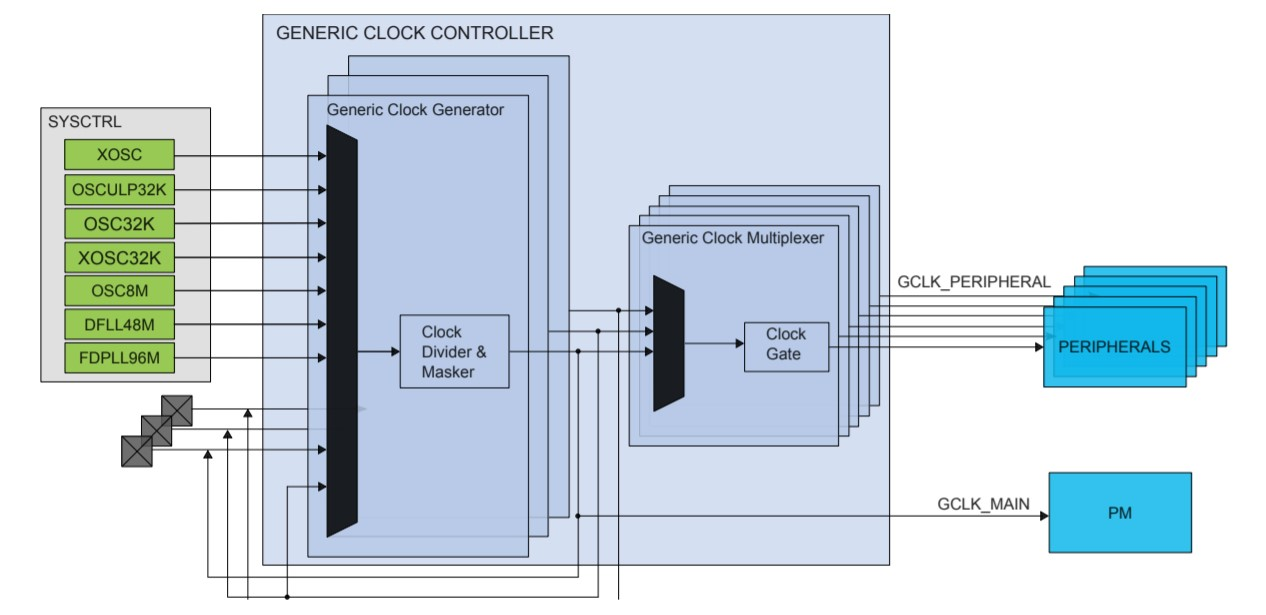
\includegraphics[width=\linewidth]{GENCLK_bloc.jpg}
		\caption{Fonctionnement du Generic Clock Controller}
	\end{figure}
	On remarque que le Generic Clock Controller est divisé en deux parties, d'une part le Generic Clock Generator configuré par le registre GENCTRL et d'autre part le Generic Clock Multiplexer configuré par le registre CLKCTRL. Le premier permet de sélectionner la source et de la diviser. Le facteur de division est définit dans un registre de taille variable en fonction du générateur pouvant aller de 5 à 16 bits. Par exemple pour le n°0 est sur 8 bits soit une division maximum par 512. Le signal divisé sur retrouve ensuite en sortie du générateur. C'est là que commence le second bloc composé de 28 multiplexeurs. Leurs entrée sont connectées à chacun des 9 générateurs et peuvent devenir le signal d'horloge du périphérique. \\ 
	Ce système de sélection est à la fois très modulaire tout en restant parfaitement optimisé. 
	
	\newpage
	\paragraph{Configuration du registre GENCTRL} 
	~~\\
	Le détail de Generic Clock Generator Control (GENCTRL) est donné dans la figure ci-dessous:\\
	\begin{figure}[H]
		\centering
		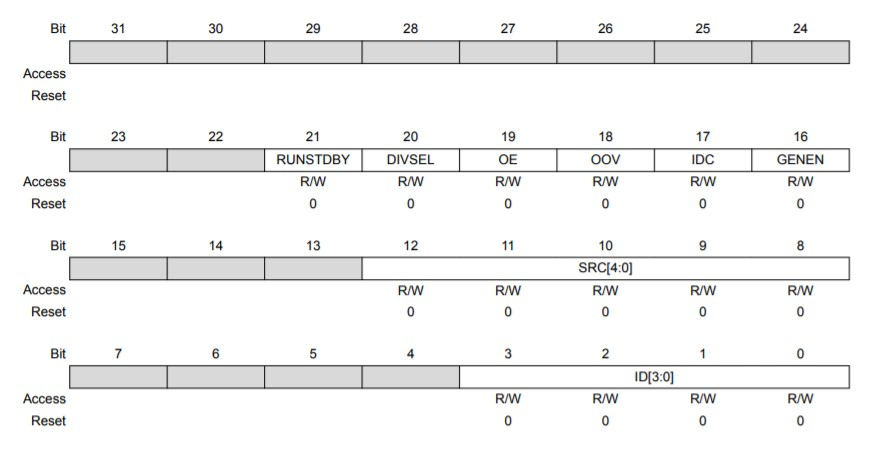
\includegraphics[width=12cm]{GENCTRL.jpg}
		\caption{Description registre GENCTRL}
	\end{figure}
	
	\begin{itemize}
		\item {\bf RUNSTDBY}: Fonctionnement en mode Standby ou non. Dans notre cas, nous voulons la désactiver donc il faut mettre {\bf 0\textless\textless21} dans ce champ.~~\\
		\item {\bf DIVSEL}: Définit le facteur de division de l’horloge. Nous ne voulons pas la diviser donc il faut mettre la valeur {\bf 0\textless\textless20} dans ce champ.~~\\
		\item {\bf OE}: Permet d’autoriser l’activation sur une sortie de GCLK. Nous ne voulons pas activer cette option donc il faut mettre la valeur {\bf 0\textless\textless19} dans ce champ.~~\\
		\item {\bf OOV}: Définit la valeur de la sortie de GCLK. Lorsque l’OE est à 0 il faut mettre également 0 dans ce champ donc la valeur {\bf 0\textless\textless18}.~~\\
		\item {\bf IDC}:Définit du rapport cyclique en cas de division impaire. Dans notre cas, il faut mettre la valeur {\bf 0\textless\textless17} dans ce champ.~~\\
		\item {\bf GENEN}: Validation ou non du générateur d’horloge. Nous voulons l’activer donc il faut mettre la valeur {\bf 1\textless\textless16} dans ce champ.~~\\
		\item {\bf SRC[4:0]}: Choix de la source d’horloge. Nous voulons choisir la source OSC8M donc d’après la datasheet il faut mettre la valeur {\bf 6\textless\textless8} dans ce champ. ~~\\
		\item {\bf ID[3:0]}: Définit le numéro du générateur que l'on configure (0 à 8). Nous choisissons la générateur 0 donc il faut mettre la valeur {\bf 0\textless\textless0}.
	\end{itemize}

	\newpage
	
	\paragraph{Configuration du registre CLKCTRL} 
	~~\\
	Ce registre permet de choisir parmis les 9 générateurs décrit précédemment. Le détail de Generic Clock Control (CLKCTRL) est donné dans la figure ci-dessous:\\
	\begin{figure}[H]
		\centering
		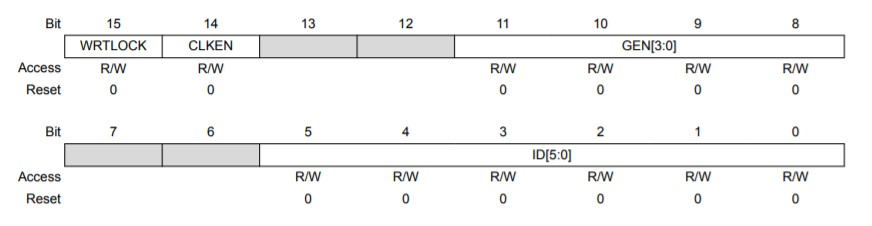
\includegraphics[width=12cm]{CLKCTRL.jpg}
		\caption{Configuration des différents bits du CLKCTRL}
	\end{figure}
	
	\begin{itemize}
		\item {\bf WRTLOCK}: Permet le verrouillage de l’horloge générique pour les générateurs 1 à 9. Nous avons choisi le générateur 0 et il n’y a pas de verrouillage donc il faut mettre {\bf 0\textless\textless15} dans ce champ.~~\\
		\item {\bf CLKEN}: Validation de l’horloge générique donc {\bf 1\textless\textless14} dans ce champ.~~\\
		\item {\bf GEN[3:0]}: Permet de choisir le générateur d’horloge d’entrée. Ici il s’agit GCLK\_GEN[0] donc il faut mettre {\bf 0\textless\textless8} dans ce champ.~~\\
		\item {\bf ID[5:0]}: Définit le périphérique vers lequel est dirigé l’horloge générique. Dans notre cas, il faut l’envoyer vers TC6 donc d’après la datasheet du SAMD21 il faut mettre la valeur {\bf 1D\textless\textless0}.~~\\
	\end{itemize}
	
	\paragraph{Code de la configuration du GCLK} ~~\\
	La configuration du GCLK traduite en langage C donne le résultat suivant:
	\begin{lstlisting}[style=CStyle]
    void config_GCLK_TC6(void){
	        Gclk *ptr_GCLK = GCLK;
	
	        ptr_GCLK->CLKCTRL.reg = GCLK_CLKCTRL_NOWRTLOCK |
							                    GCLK_CLKCTRL_CLKEN |
							                    GCLK_CLKCTRL_GEN_GCLK0 |
							                    GCLK_CLKCTRL_ID_TC6_TC7 ;
	
	        ptr_GCLK->GENCTRL.reg = GCLK_GENCTRL_NORUNSTDBY |
							                    GCLK_GENCTRL_NODIVSEL |
							                    GCLK_GENCTRL_NOOE |
							                    GCLK_GENCTRL_NOOOV |
							                    GCLK_GENCTRL_NOIDC |
							                    GCLK_GENCTRL_GENEN |
							                    GCLK_GENCTRL_SRC_OSC8M |
						        	            GCLK_GENCTRL_ID(0);
    }
	\end{lstlisting}
	
	\subsubsection{Configuration du Power Manager(PM)} 
	Les périphériques communiques avec le microprocesseur via un bus synchrone. Son horloge est délivrée par le Power Manager (PM).
	Il gère trois domaines d'horloge, une pour le CPU, une pour le bus AHB à destination de la mémoire et trois clocks pour le bus APB à destination des périphériques.
%	\begin{figure}[H]
%		\centering
%		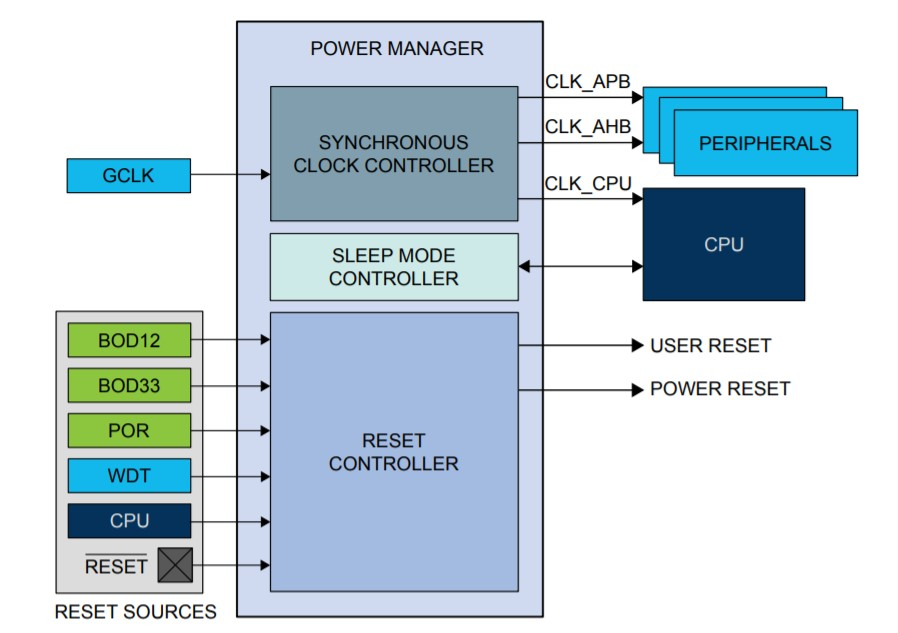
\includegraphics[width=0.6\linewidth]{PM_bloc.jpg}
%		\caption{Structure du Power Manager}
%	\end{figure}
	Le "Synchronous Clock Controller" prend en entré la sortie de GCLK et sort 3 horloges pour les 3 bus internes du microprocesseur: APBA, APBB et APBC.\\
%	\begin{figure}[H]
%		\centering
%		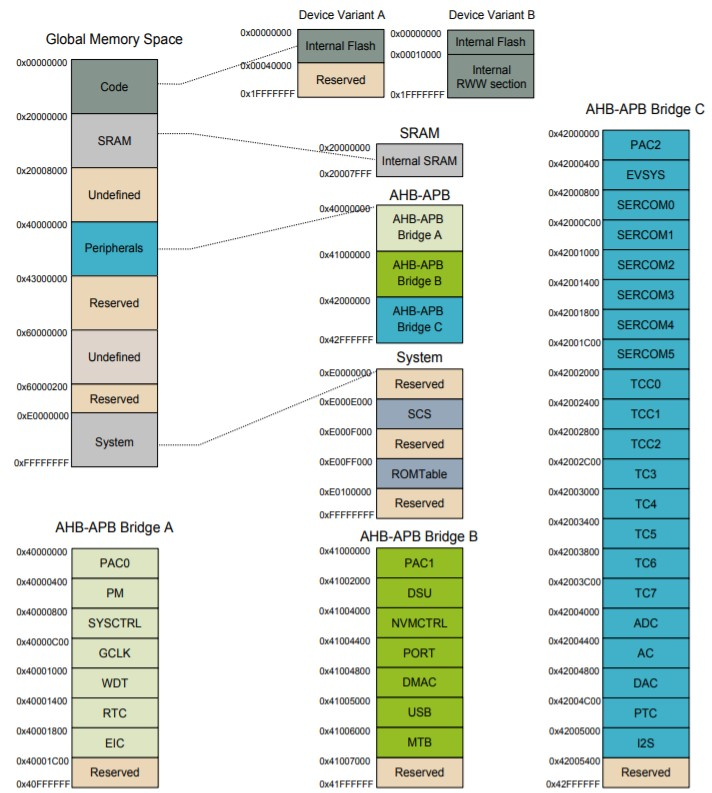
\includegraphics[width=0.8\linewidth]{product mapping_SAMD21.jpg}
%		\caption{Cartographie des produits Atmel SAM D21}
%	\end{figure}
	D'après la cartographie des produits, le Timer TC6 est placé sur le bus APBC. Il faut donc configurer les registres:
	\begin{itemize}
		\item {APBCSEL}
		\item {APBCMASK}
		\item {CPUSEL}
	\end{itemize}
Ils sont respectivement en charge du facteur de division appliqué sur l'horloge de APBC, du masque d'activation et du facteur de division appliqué sur l'horloge du CPU.
	\newpage
	\paragraph{Configuration du registre APBCSEL} 
	~~\\
	Le registre APBA Clock Select (APBCSEL) ne contient qu'un seul champ:\\
	\begin{figure}[H]
		\centering
		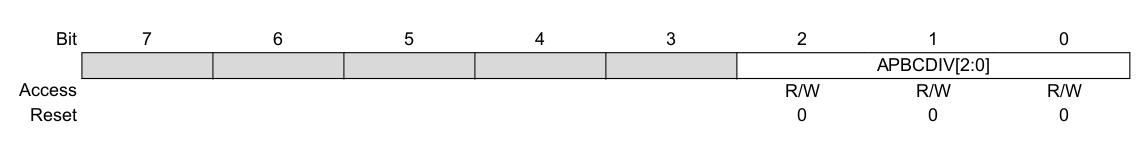
\includegraphics[width=0.9\linewidth]{APBCSEL.jpg}
		\caption{Description registre APBCSEL}
	\end{figure}
	
	\begin{itemize}
		\item {\bf APBCDIV[2:0]}: Définit le facteur de division de l'horloge d'entrée GCLKMAIN. On choisit la division par 1 donc il faut mettre {\bf 0\textless\textless0}.~~\\
	\end{itemize}
	
	\paragraph{Configuration du registre APBCMASK} 
	~~\\
	Le registre APBC Mask (APBCMASK) contient les validations d'horloge bus pour tous les périphériques connectes sur le bus APBC.
	\begin{figure}[H]
		\centering
		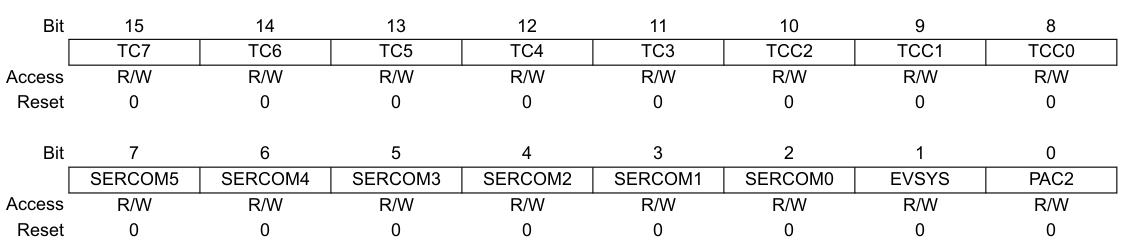
\includegraphics[width=0.9\linewidth]{APBCMASK.jpg}
		\caption{Extrait de description registre APBCMASK}
	\end{figure}
	Les bits 20:0 permettent de stopper les différentes horloges bus de APBC s’ils sont mis à zéro ou bien de les activer s’ils sont mis à un.
	\begin{itemize}
		\item {\bf TC6}: Ici on veut activer l’horloge bus pour TC6 donc il faut mettre {\bf 1\textless\textless14}.~~\\
	\end{itemize}
	
	\paragraph{Configuration du registre CPUCSEL} 
	~~\\
	Le registre CPU Clock Select (CPUSEL) ne contient qu'un seul champ:
	\begin{figure}[H]
		\centering
		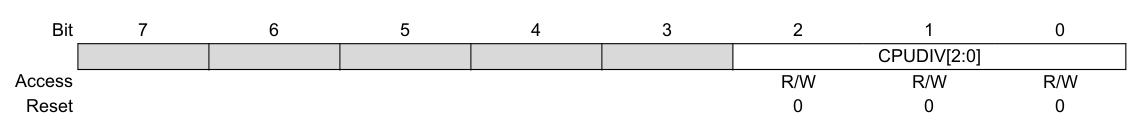
\includegraphics[width=0.9\linewidth]{CPUSEL.jpg}
		\caption{Description registre CPUSEL}
	\end{figure}
	\begin{itemize}
		\item {\bf CPUDIV[2:0]}: Permet de définir de facteur de division de l'horloge du CPU par rapport à GCLKMAIN. On choisit la division par 1 donc il faut mettre {\bf 0\textless\textless0}.~~\\
	\end{itemize}
	
	\paragraph{Code de la configuration du PM} ~~\\
	La configuration du PM traduite en langage C donne le résultat suivant:
	\begin{lstlisting}[style=CStyle]
void config_PM(void){
	    Pm *ptr_PM = PM;
	
	    ptr_PM -> CPUSEL.reg = PM_CPUSEL_CPUDIV_DIV1;
	    ptr_PM -> APBCSEL.reg = PM_APBCSEL_APBCDIV_DIV1;
	    ptr_PM -> APBCMASK.reg |= PM_APBCMASK_TC6;
}
	\end{lstlisting}
	
	\subsubsection{Configuration des ports d'E/S parallèles} 
	Le nombre de broches du microprocesseur est limité: le SAMD21 en possède 64, un nombre bien inférieur à la somme des entrées/sorties de tous les périphériques. Il faut donc multiplexer les entrées ou les sorties des périphériques via les ports d’entrée/sortie A et B. Dans un premier il nous faut donc déterminer quelles broches, et dans quel multiplexeur il est possible d’observer le signal WO[0] du TC6. D’après la table de multiplexage présente dans la datasheet du SAMD21 (extrait figure \ref{fig:MUX_io}), ce signal est disponible sur 2 pins : PB02 et PB16. Cependant la pin PB16 est déjà utilisé pour d’autres fonctions, il est donc préférable de prendre la \textbf{broche PB02}. Il faudra sélectionner le \textbf{multiplexeur E}.
	\begin{figure}[H]
		\centering
		\includegraphics[width=\linewidth]{MUX_io}
		\caption{Extrait tableau multiplexage fonction port}
		\label{fig:MUX_io}
	\end{figure}
    Pour accéder a la sortie WO[0] de TC6, il faudra configurer :
    \begin{itemize}
		\item {Registre \bf DIRSET} pour choisir la broche PB02 en sortie
		\item {Registre \bf PMUX} pour choisir le multiplexage de type E
		\item {Registre \bf PINCFG} pour valider le multiplexage choisi
	\end{itemize}
	
	\paragraph{Configuration du registre DIRSET} 
	~~\\
	Le registre Data Direction Set (DIRSET) permet à l'utilisateur de définir une ou plusieurs broches d'E/S en sortie. Ce registre sert à mettre à 1 en bits correspondants dans le registre DIR. Le registre DIR contient le configuration de chacune des pattes du port A ou B.
	\begin{figure}[H]
		\centering
		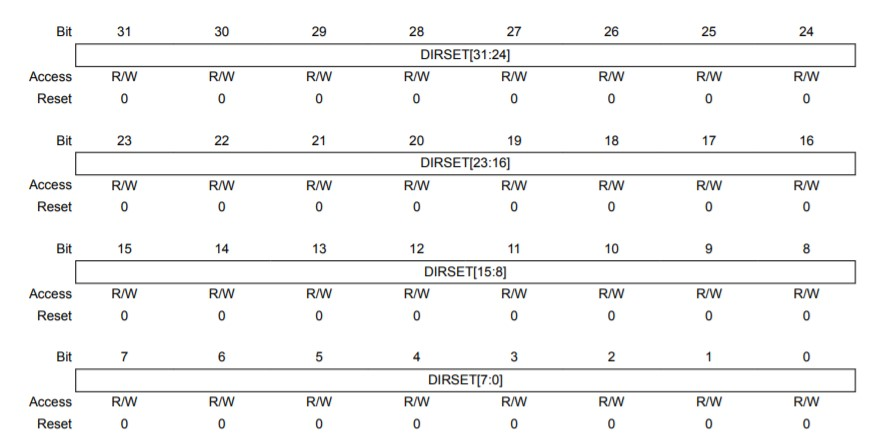
\includegraphics[width=0.92\linewidth]{DIRSET.jpg}
		\caption{Description registre CPUSEL}
	\end{figure}
	\begin{itemize}
		\item {\bf DIRSET[31:0]}: Le bit à 0 n'a aucun effet. Le bit à 1 configure la broche d'E/S comme une sortie. Pour le port B, il faut configurer la patte 2 en sortie donc il faut mettre {\bf 1\textless\textless2}.
	\end{itemize}
	\newpage
	\paragraph{Configuration du registre PMUX} 
	~~\\
	Il y a jusqu'à 16 registres de multiplexage périphérique dans chaque groupe, un pour chaque ensemble de deux lignes d'E/S. Le n désigne le numéro de l'ensemble des lignes d'E/S.
%	\begin{figure}[H]
%		\centering
%		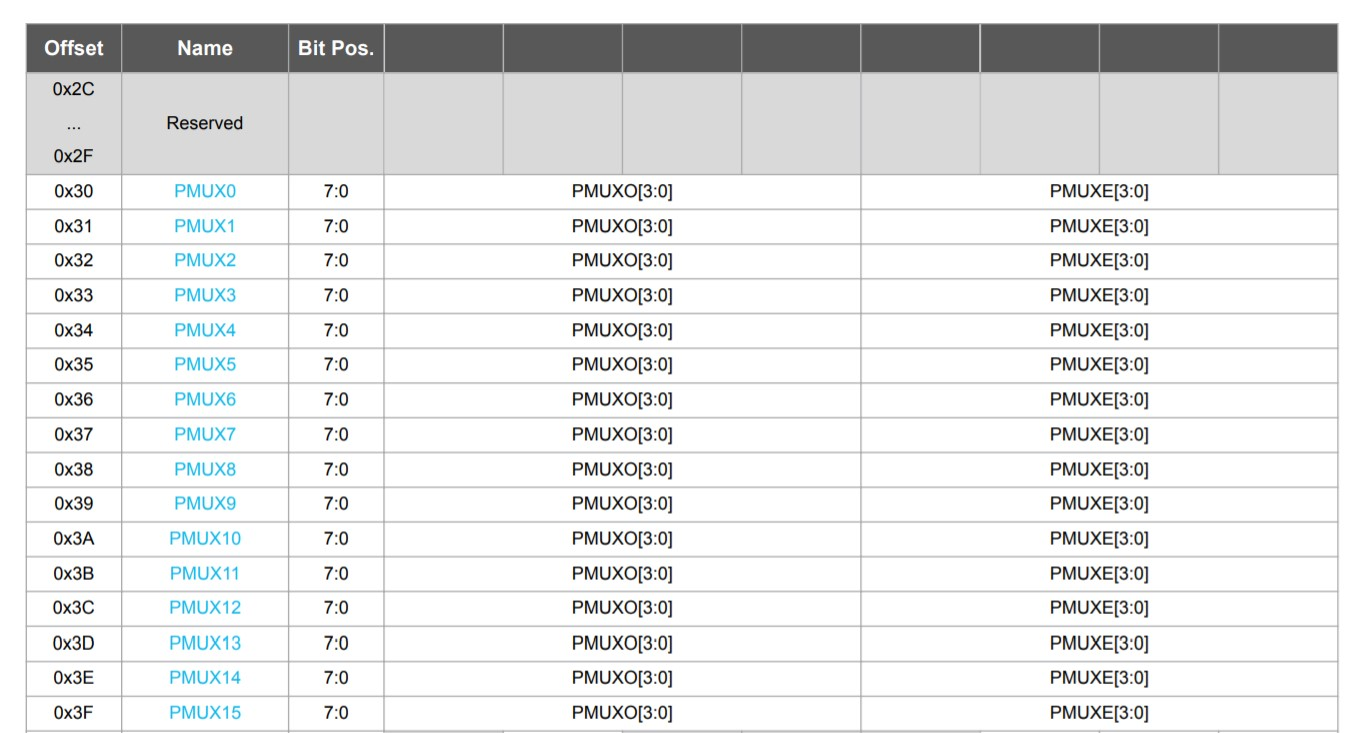
\includegraphics[width=0.9\linewidth]{Registre du PMUXn.jpg}
%		\caption{Registre du PMUXn}
%	\end{figure}
	Le registre  Peripheral Multiplexing n (PMUXn) est composé de 16 octets, chacun composé de 2 parties : 4 bits pour les pins impaires, 4 bits pour les pins paires. Ainsi PMUX0 contient le multiplexage des pins 0 (paire) et 1 (impaire). La pin 2 est alors la partie paire de PMUX1.  
	\begin{figure}[H]
		\centering
		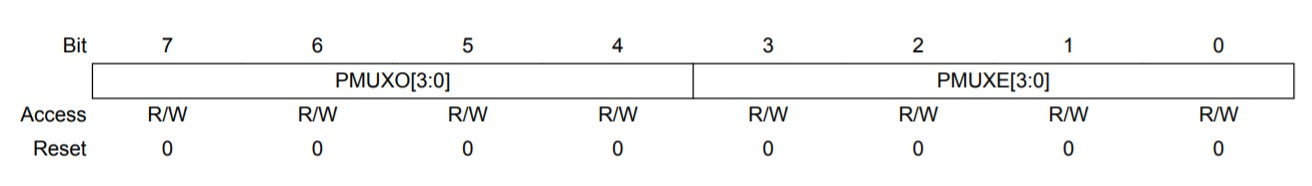
\includegraphics[width=0.9\linewidth]{PMUX.jpg}
		\caption{Description registre PMUXn}
	\end{figure}
	
	\begin{itemize}
		\item {\bf PMUXE[3:0]}: 0x0 étant le multiplexage A, et 0x8 le I. On spécifie alors le multiplexage à mettre en place : E, donc il faut mettre la valeur {\bf 0x4\textless\textless0}.
	\end{itemize}
	
	\paragraph{Configuration du registre PINCFG} 
	~~\\
	Enfin, il faut activer la broche PB02 en passant par les registres Pin Configuration (PINCFG).Ils sont définis ainsi:   
	\begin{figure}[H]
		\centering
		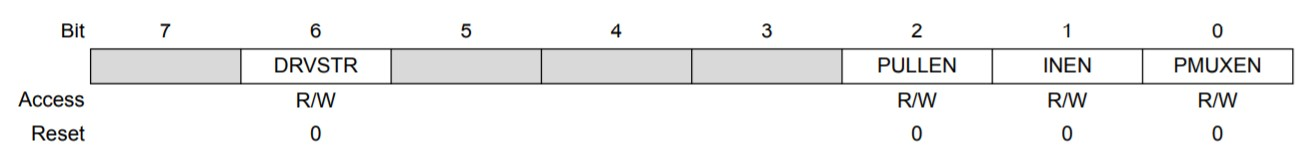
\includegraphics[width=0.9\linewidth]{PINCFGn.jpg}
		\caption{Description registre PINCFGn}
	\end{figure}
	
	\begin{itemize}
		\item {\bf DRVSTR}: Contrôle la force du driver de sortie. 1 pour fort, 0 pour normal. Ne nous concerne pas ici donc il faut mettre {\bf 0\textless\textless6} dans ce champ.~~\\
		\item {\bf PULLEN}: Active ou non un la résistance pull-up ou pull-down interne d'une broche d'E/S configurée en entrée. Ne nous concerne pas ici, donc {\bf 0\textless\textless2}.~~\\
		\item {\bf INEN}: : Validation de la patte comme une entrée. On considère ici une sortie donc il faut mettre {\bf 0\textless\textless1} dans ce champ.~~\\
		\item {\bf PMUXEN}: Validation ou non le multiplexage E mis en place par le registre PMUX correpondant donc il faut mettre {\bf 1\textless\textless0}.~~\\
	\end{itemize}
	\newpage
	\subsubsection{Configuration du périphérique} 
	Nous utiliserons pour cette partie le Timer Counter 6 (TC6) configuré dans le mode 16 bits. Pour générer un signal de fréquence 1kHz, il faut programmer les registres:
	
	\paragraph{Code de la configuration du PORT} ~~\\
	La configuration du PORT traduite en langage C donne le résultat suivant:
	\begin{lstlisting}[style=CStyle]
void config_PORT(void){
	    Port *ptr_port = PORT ;
	
	    ptr_port -> Group[1].DIRSET.reg = PORT_PB02; 
	    ptr_port -> Group[1].PMUX[2/2].reg = PORT_PMUX_PMUXE_E;
	    ptr_port -> Group[1].PINCFG[2].reg = PORT_PINCFG_DRVSTR_NO |
	                                         PORT_PINCFG_PULLEN_NO |
	                                         PORT_PINCFG_INEN_NO |
	                                         PORT_PINCFG_PMUXEN;
}
	\end{lstlisting}
	
	\subsubsection{Configuration du périphérique Timer Counter} 
	Nous utiliserons pour cette partie le Timer Counter 6 (TC6) configuré dans le mode 16 bits.\\
	Pour générer un signal de fréquence 1kHz, il faut programmer le registre:
	\begin{itemize}
		\item {CTRLA}
		\item {CTRLBLR}
		\item {CTRLC}
		\item {CC0}
	\end{itemize}
	\paragraph{Configuration du registre CTRLA} 
	~~\\
	Le détail de Control A (CTRLA) est donné dans la figure ci-dessous :
	\begin{figure}[H]
		\centering
		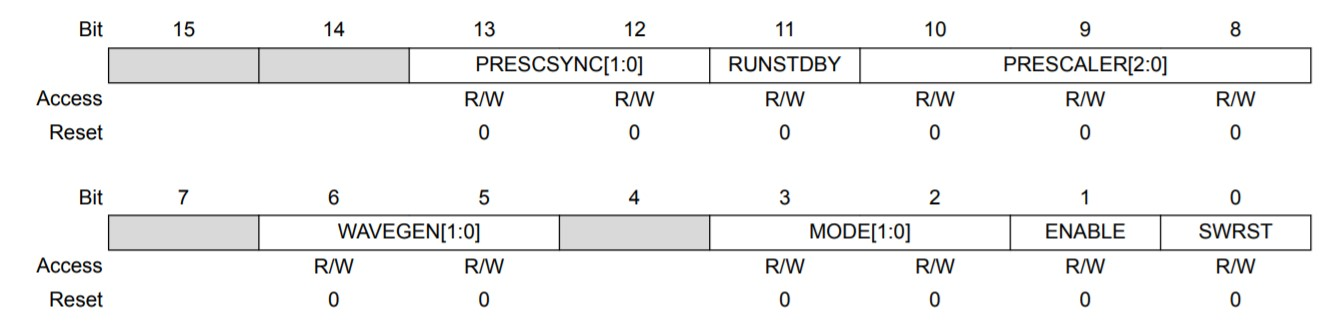
\includegraphics[width=0.9\linewidth]{ControlA.jpg}
		\caption{Description registre CTRLA}
	\end{figure}
	
	\begin{itemize}
		\item {\bf PRESCSYNC[1:0]}: Le registre de comptage est piloté par une horloge issue de GCLK\_TC via un prescaler. Il faut donc mettre la valeur {\bf 1\textless\textless12}.~~\\
		\item {\bf RUNSTDBY}: Définit le fonctionnement du TC en mode STANDBY. Il n’y a pas d’intérêt à garder le TC actif en veille donc {\bf 0\textless\textless11}.~~\\
		\item {\bf PRESCALER[2:0]}: Applique un facteur de division à l’horloge d’entrée entre 1 et 1024. Il ne sera pas nécessaire de diviser au préalable l’horloge donc on garde un prescaler de 1 alors {\bf 0\textless\textless8}.~~\\
		\item {\bf WAVEGEN[1:0]}: Sélectionne le mode de fonctionnement du compteur. Le mode MFRQ est utilisé, il faut donc {\bf 1\textless\textless5}.~~\\
		\item {\bf MODE[1:0]}: Sélectionne le mode de comptage pour le compteur, c’est-àdire le nombre de bits de comptage : 8, 16 ou 32 bits. Il nous faut ici compter 4000 valeurs (de 0 à 3999) d’après le modèle présenté en début de section. C’est donc le mode 16 bits qui est choisi, alors {\bf 0\textless\textless2}.~~\\
		\item {\bf ENABLE}: Valide le timer ou non. Ici nous voulons le valider donc il faut mettre la valeur {\bf 1\textless\textless1}.~~\\
		\item {\bf SWRST}: Nous ne voulons pas de RESET du Timer donc il faut mettre la valeur {\bf 0\textless\textless0}.~~\\
	\end{itemize}
	
	\newpage
	\paragraph{Configuration du registre CTRLBCLR} 
	~~\\
	Le détail de Control B Clear (CTRLBCLR) est donné dans la figure ci-dessous :
	\begin{figure}[H]
		\centering
		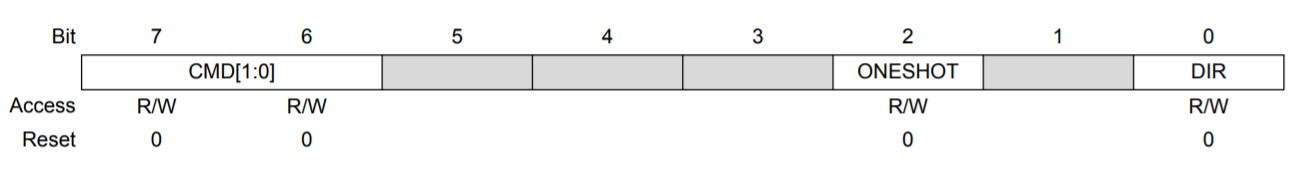
\includegraphics[width=0.9\linewidth]{CTRLBCLR.jpg}
		\caption{Configuration des différents bits du CTRLBCLR}
	\end{figure}
	
	\begin{itemize}
		\item {\bf CMD[1:0]}: Sélectionne la commande lors du prochain cycle de GCLK du TC: NONE, RETRIGGER ou STOP. Aucun comportement particulier n’est souhaité, on place alors NONE {\bf 0\textless\textless6}.~~\\
		\item {\bf ONESHOT}: Le One-Shot stop le compteur lors d’un débordement du compteur (inférieur à 0 ou supérieur à la valeur maximale). Placé ce bit à 1 stop cette fonctionnalité. On veut le désactiver donc il faut mettre la valeur {\bf 1\textless\textless2}.~~\\
		\item {\bf DIR}: Paramètre le sens de comptage : incrémentation(1) ou décrémentation(0). On choisit le mode incrémention donc {\bf 1\textless\textless0}.~~\\
	\end{itemize}
	
	\paragraph{Configuration du registre CTRLC} 
	~~\\
	Le détail de Control C (CTRLC) est donné dans la figure ci-dessous :
	\begin{figure}[H]
		\centering
		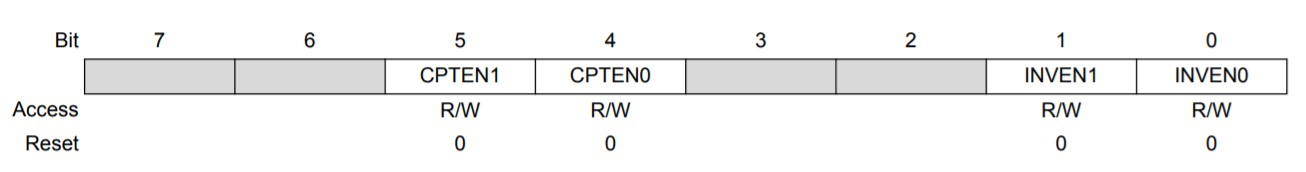
\includegraphics[width=0.9\linewidth]{CTRLC.jpg}
		\caption{Configuration des différents bits du CTRLC}
	\end{figure}
	
	\begin{itemize}
		\item {\bf CPTENx}: Autorise la capture sur les channel 1 et 0. On veut désactiver le mode capture 1 et capture 0 donc il faut mettre la valeur {\bf 0\textless\textless5} et {\bf 0\textless\textless4}.~~\\
		\item {\bf INVENx}: Inverse les sorties WO[1] et WO[0] lorsque ces bits sont à 1. On ne veut pas inverser la sortie WO[1] et WO[0] donc il faut mettre la valeur {\bf 0\textless\textless1} et {\bf 0\textless\textless0}.~~\\
	\end{itemize}
	
	\paragraph{Configuration du registre CC0} 
	~~\\
	Ce registre permet de définir la demi période CC0 du signal W0[0]. \\
	D’après les calculs présenté précédemment, pour générer un signal de fréquence 1kHz, la valeur chargée dans le registre CC0 est donc 3999.\\
	
	\newpage 
		\paragraph{Code de la configuration du TC6} ~~\\
	La configuration du TC6 traduite en langage C donne le résultat suivant:
	\begin{lstlisting}[style=CStyle]
void config_TC6(void){
	    Tc *ptr_TC = TC6 ;
	
	    ptr_TC -> COUNT16.CTRLA.reg = TC_CTRLA_PRESCSYNC_PRESC |
	                                  TC_CTRLA_NORUNSTDBY |
	                                  TC_CTRLA_PRESCALER_DIV1 |
	                                  TC_CTRLA_WAVEGEN_MFRQ |
	                                  TC_CTRLA_MODE_COUNT16 |
	                                  TC_CTRLA_ENABLE |			
	                                  TC_CTRLA_NOSWRST;
	    ptr_TC -> COUNT16.CTRLC.reg = TC_CTRLC_NOCPTEN0 |
	                                  TC_CTRLC_NOCPTEN1 |
	                                  TC_CTRLC_NOINVEN0 |
	                                  TC_CTRLC_NOINVEN1;
	    ptr_TC -> COUNT16.CTRLBCLR.reg = TC_CTRLBCLR_CMD_NONE |
	                                     TC_CTRLBCLR_ONESHOT |
                                    	 TC_CTRLBCLR_DIR;
    	ptr_TC -> COUNT16.CC[0].reg = 3999;
    	ptr_TC -> COUNT16.CTRLA.reg |= TC_CTRLA_ENABLE;
}
	\end{lstlisting}
	
	\subsection{Test et validation}
	La traduction des spécifications ci-dessus sont traduite en langage C et implantés sur la carte. Le programme complet de cette partie est disponible en annexe.\\
	A l’aide d’un oscilloscope, on visualise le signal de sortie sur la pin PB02 paramétrée précédemment. Le signal en sortie du TC6 présenté en figure ci-dessous:
	\begin{figure}[H]
		\centering
		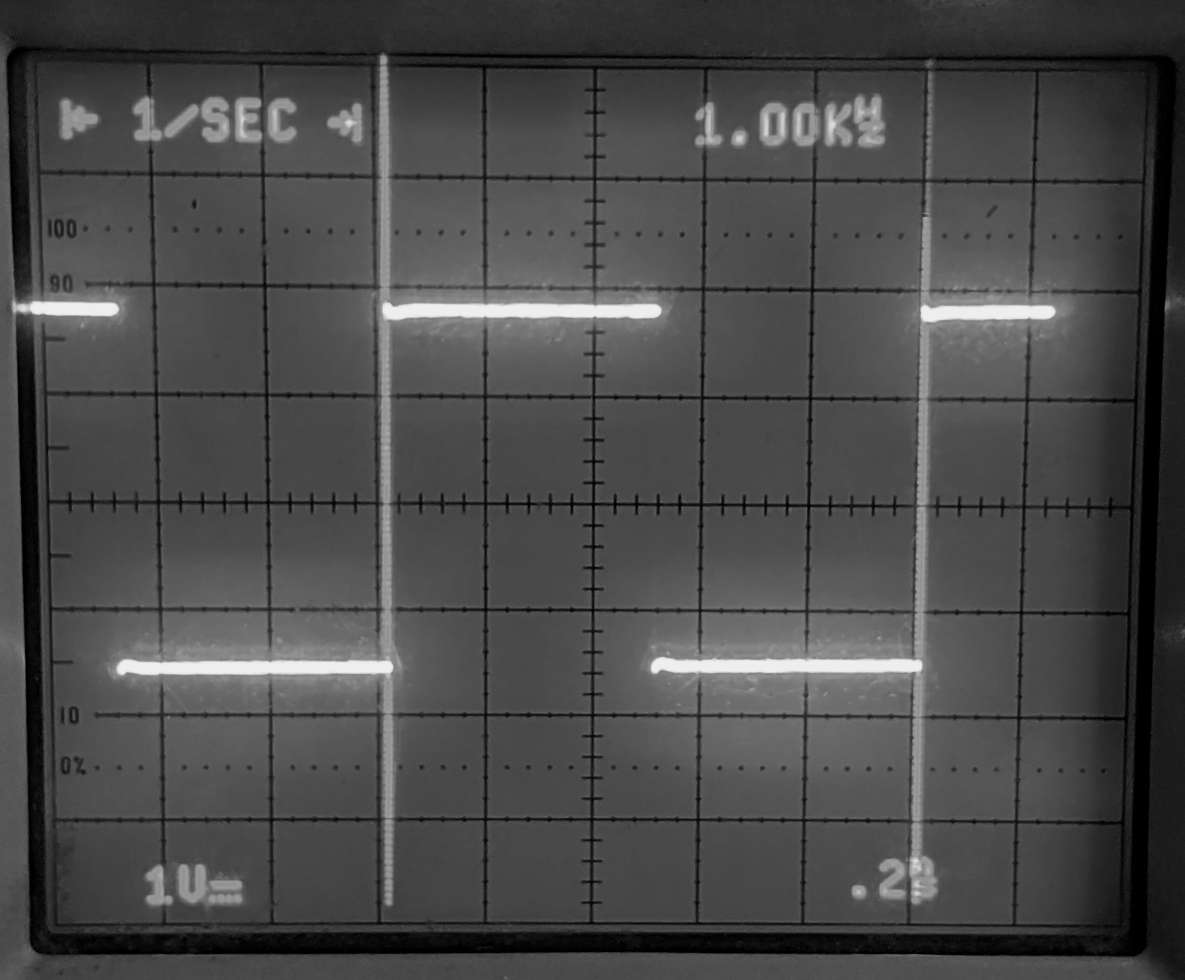
\includegraphics[width=0.6\linewidth]{chrono_valide_etape2.jpg}
		\caption{Signal de sortie du TC6}
	\end{figure}
	On obtient bien un signal carré de fréquence 1kHz comme signal en sortie du TC6.
	


	
	\newpage
	
	
	\section{Fonction sous interruption}
	Les interruptions sont des outils essentiels pour concevoir des systèmes réactifs (en: responsive)  dès lors qu'ils doivent exécuter des opérations logicielles et matérielles simultanément. Avant de présenter le fonctionnement et la configuration du système d'interruption du Cortex-M il est préférable de donner un aperçu du problème.
	\subsection{Présentation du problème}
	L'environnement avec lequel interagi le microcontrôleur est dit asynchrone. Il ne peut à priori par connaître l'instant d'apparition d'un événement. Il est alors obligé de le scruter fréquemment pour être averti rapidement d'un changement. C'est précisément ce que fait l'étape 1. La lecture du bouton est placée dans une boucle infinie, si l'utilisateur appui sur ce denier l'état de la led est modifié. Bien que ce programme soit inefficace, il fonctionne bien et offre une faible latence. Ce mode de fonctionnement est appelé "polling". Le problème survient dès lors qu'une tâche logicielle est ajoutée au programme. Le processeur n'est plus seulement occupé à contrôler l'état du bouton mais également à exécuter une autre partie du programme. La réactivité n'est alors plus garantie. Dans certains cas, si la tâche logicielle est importante, le changement d'état du bouton pourra être invisible pour le programme.
	\begin{figure}[H]
		\centering
		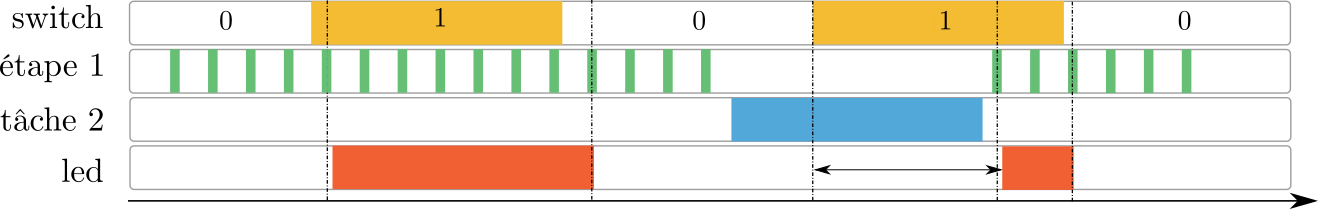
\includegraphics[width=\linewidth]{polling_task}
		\caption{Ordonnancement tâches avec polling}
	\end{figure}
	La figure ci-dessus représente l'exécution \footnote{Aucune échelle précise n'est choisi le but étant une simple présentation fonctionnelle.} d'un programme comme celui de l'étape 1 auquel une seconde tâche a été ajoutée (tâche 2).  Deux cas sont illustrés dans cet exemple. Le premier, à gauche, correspond au bon déroulement, le processeur lit de manière successive l'état du switch (étape 1), lorsque une lecture vaut '1' l'état de la led est mis à '1' et même chose pour '0'. Une petite (latence) est présente mais elle sera généralement négligée. Dans le second cas, à droite, la tâche 2 est en cours d'exécution est empêche la lecture du bouton. Une fois terminée la mise à jours de la led peut s'opérer comme précédement. L'exécution de la tâche 2 a générer un retard qui n'est cette fois-ci plus négligeable du point de vue de l'utilisateur. Si la tâche 2 avait durée un instant de plus le système n'aurait pas réagi à la stimulation. Un tel cas ne doit, en aucun cas, se produire pour un système dont la sécurité est critique.\\
	En pratique ce problème survient fréquemment. Les interactions utilisateurs, tel que l'appuis sur un bouton, sont relativement lentes comparés à la vitesse de fonctionnement des processeurs. Un "polling" pourra suffire dans certains cas. Mais pour ce qui est des événements matériels, comme un timer ou un protocole série, la situation est plus critique. Il n'y a alors pas d'autres solutions que d'utiliser une interruption. De manière générale les logiciels utilisant des interruptions fonctionnent plus efficacement que ceux basés sur le "pooling". Aucun temps n'est perdu à contrôler l'apparition d'un événement. L'approche par déclenchement sur évènements (en: even-trigger) offre également une meilleur réactivité. \cite{ARM_book}
	\subsection{Fonctionnement d'une interruption }
	Une interruption est définie comme une suspension temporaire de l'exécution d'un programme informatique par le microprocesseur afin d'exécuter un programme prioritaire (routine d'interruption). La dite suspension est déclenchée par une source externe. \\
	La gestion d'une interruption s'effectue comme tel : pause du programme, sauvegarde du contexte, identification de la routine d'interruption à exécuter (en fonction de ma source), exécution de la routine et rétablissent du contexte. Ces actions sont gérées par le NVIC, Nest Vectored Interrupt Controler faisant l'interface entre les périphériques et le CPU.
	\begin{figure}[H]
		\centering
		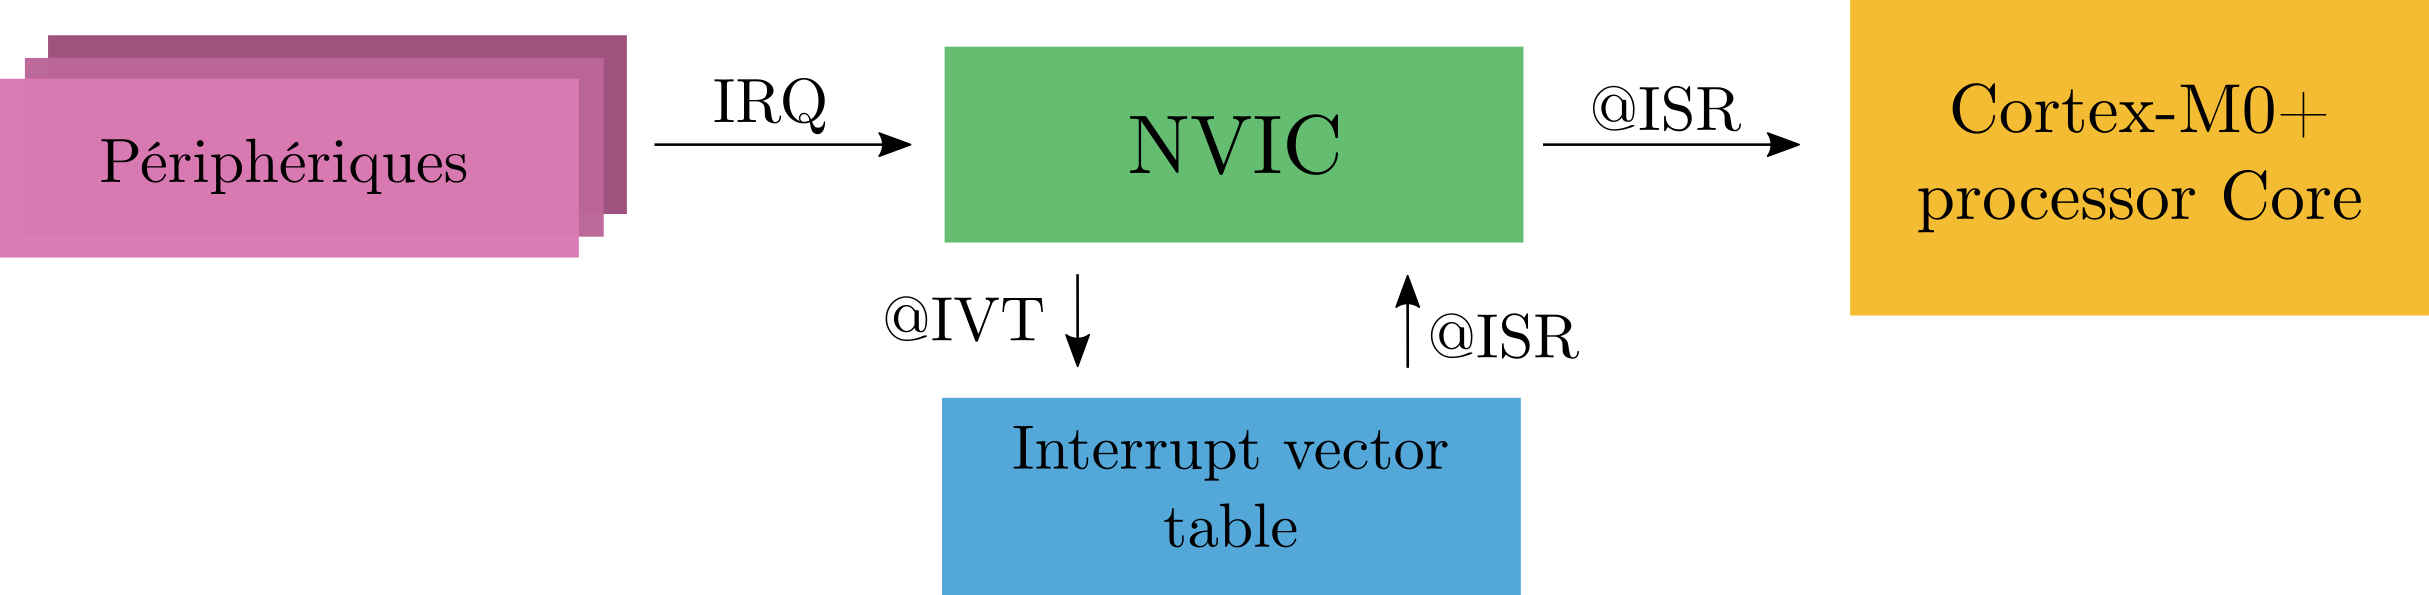
\includegraphics[width=0.9\linewidth]{NVIC}
		\caption{Schéma bloc NVIC}
		\label{fig:NVIC}
	\end{figure}
	
	
	Lorsqu'une interruption x se produit, la demande d'interruption (IRQ) est envoyée au NVIC. Si le NVIC accepte la demande, l'étape suivante du NVIC consiste à trouver l'adresse de départ de la routine d'interruption (@ISR). Cette adresse est stockée dans la table de vecteurs d'interruption (IVT). Le NVIC utilise le numéro d'interruption x pour calculer l'adresse de l'exception dans la table des vecteurs d'interruption. Il utilise ensuite le contenu de cette adresse mémoire pour exécuter le gestionnaire d'exception. Le compteur de programme est alors chargé avec l'adresse de l'ISR et le CPU commence à exécuter la routine d'exception.
	Un rappel du vocabulaire utilisé dans la figure \ref{fig:NVIC}.
	
	\begin{table}[H]
		\centering
		\begin{tabular}{|c|l|}
			\hline
			@ & adresse mémoire \\
			\hline
			IRQ & Interrupt Service Routine \\
			\hline
			NVIC & Nest Vectored Interrupt Controler \\
			\hline
			IVT & Interrupt Vector table \\
			\hline
			ISR & Interrupt Service Rotine \\
			\hline
		\end{tabular}
	\caption{Terminologie mécanisme d'interruption}
	\end{table}
	La table des vecteurs d'interruptions, est une structure de données et, comme son nom l'indique, un tableau contenant des vecteurs. En programmation embarquée, un vecteur désigne une adresse mémoire. Par conséquent, une table de vecteurs est une table contenant des adresses mémoire. \textbf{La table des vecteurs d'interruption contient les adresses (pointeurs de fonction) des routines d'interruption et des fonctions de gestion des exceptions.} Les exceptions désignent les évènements en mesure d'interrompre le déroulement normal du programme pour effectuer une courte tache. Les interruptions sont donc partie des exceptions. Elles ne sont pas les seules le processeur lui même peut déclencher le mécanisme d'exception lorsque on lui demande de faire quelque chose qu’il ne parvient pas à faire. Par exemple la lecture d'un mot de 32 bits à une adresse impaire provoquera une exception à l'exécution.
	
	\subsection{Configuration interruption}
	Pour qu'une interruption se produise il faut que le périphérique soit configuré de sorte à réagir à l'occurrence d'un événements spécifique. Dans le contexte du projet nous devons calculer le gabarit toutes les 1 ms. Cette partie présente la configuration à effectuer pour que le timer TC6 déclenche une routine d'interruption contenant la fonction calcul gabarit. Elle détaillera également l'autorisation de l'interruption par le NVIC.
	\subsubsection{Timer TC6}
	L'activation de l'interruption sur le périphérique TC6 est documentée en détaille dans la datasheet. \cite{data} Chaque source d'interruption est associée à un drapeau d'interruption. Le drapeau d'interruption (en: interrupt flag), dans le registre (INTFLAG), est activé lorsque la condition d'interruption en vrai. Chaque interruption peut être activée individuellement en écrivant un '1' au bit correspondant dans le registre d'activation Interrupt Enable Set (INTENSET) et désactivée en écrivant un '1' au bit correspondant dans le registre de désactivation Interrupt Enable Clear (INTENCLR).	Le registre INTENSET se présente comme tel :
	\begin{figure}[H]
		\centering
		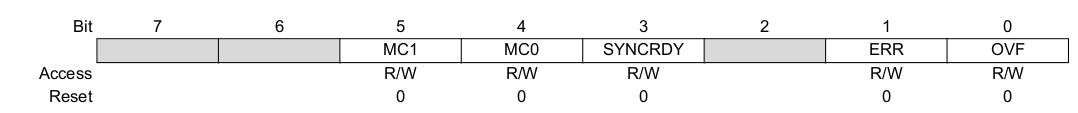
\includegraphics[width=\linewidth]{reg_intenset}
		\caption{Registre INTENSET}
		\label{fig:INTENSET}
	\end{figure}
	Ayant programmé le timer en mode MFRQ dans la partie précédente, seul le bit 4 nous intéresse. Il est chargé à '1' pour activer l'interruption sur correspondance de COUNT et MC0. L'implémentation en C est intuitive :
	\begin{lstlisting}[style=CStyle]
	void configure_TC6_IT(void){
		Tc *ptr_TC = TC6;
		ptr_TC->COUNT16.INTENSET.reg = TC_INTFLAG_MC0;
	}
	\end{lstlisting}
	
	Comme l'indique la datasheet après la configuration du périphérique il faut activer l'interruptions correspondante dans NVIC.
	\begin{quotation}
		"The interrupt request line is connected to the Interrupt Controller. In order to use interrupt requests of this peripheral,
	the Interrupt Controller (NVIC) must be configured first." \cite{data}(page 557)
	\end{quotation}
	
	\subsubsection{NVIC}
	Le NVIC est un élément interne au processeur. La documentation de Microchip donne pour chaque périphérique le numéro d'interruption associée mais renvoit à la documentation de Arm pour la configuration du NVIC. Le numéro du TC6 est 21. Comme nous avons pu l'évoquer plus haut le NVIC peut accepter ou non les interruptions provenant des périphériques. Il consulte pour cela un registre nommé NVIC\_ISER contenant un seul champ de 32 bits SETENA littéralement set enable. L'extrait de la documentation \cite{ARMv6} Arm ci-dessous nous donne la valeur des bits à charger.
	\begin{figure}[H]
		\centering
		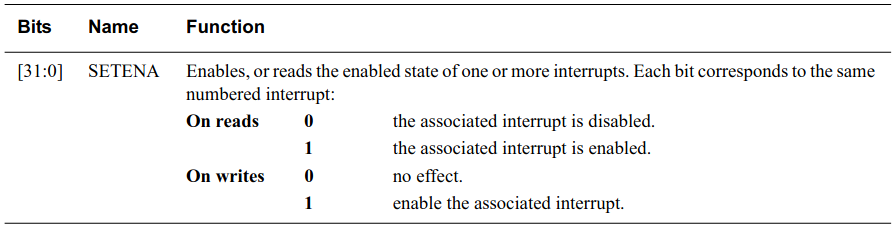
\includegraphics[width=0.8\linewidth]{ISER}
		\caption{Registre NVIC\_ISER ARMv6-M}
		\label{fig:ISER}
	\end{figure}
	Ce registre permet de lire l'activation ou d'activer l'interruption sur chaque ligne. A noter : il faut utiliser un autre regiqtre pour la désactivation, écrire un '0' n'aura aucun effet. \textbf{Nous devons dans notre cas placer un '1' sur le bit 21.} Cette configuration est grandement simplifiée par l'ASF. Mais il est essentiel de comprendre et de retenir qu'une activation supplémentaire au périphérique est nécessaire. Le code ajouter à la fonction main est le suivant :
	\begin{lstlisting}[style=CStyle]
		system_interrupt_enable(SYSTEM_INTERRUPT_MODULE_TC6);\end{lstlisting}
	L'appel de cette fonction est simple et permet l'abstraction du matériel. Le paramètre passé est le numéro d'interruption \texttt{TC6\_IRQn} comme le montre la définition dans \texttt{system\_interrupt\_features.h}
	\begin{lstlisting}[style=CStyle]
	SYSTEM_INTERRUPT_MODULE_TC6 = TC6_IRQn\end{lstlisting}
	\texttt{TC6\_IRQn} est défini plus haut et dépend de la cible utilisée dans notre cas le SAMD21J18A. 
	\begin{lstlisting}[style=CStyle]
	 TC6_IRQn                 = 21 \end{lstlisting}
	Sa valeur est bien 21. Nous venons d'observer la cohérence entre la datasheet et l'ASF. Pour finaliser le raisonnement regardeons l'implémentation de la fonction \texttt{system\_interrupt\_enable()}.
	\begin{lstlisting}[style=CStyle]
	static inline void system_interrupt_enable(
	const enum system_interrupt_vector vector)
	{
		NVIC->ISER[0] = (uint32_t)(1 << ((uint32_t)vector & 0x0000001f));
	}\end{lstlisting}
	Cette fonction est particulièrement intéressante d'un point de vue pédagogique par l'utilisation de static, inline et du masquage sur le vecteur. D'un point de vue fonctionnel, elle place un '1' décalé du numéro d'interruption sur le registre ISER de NVIC. C'est précisément ce qui doit être fait pour activer les interruptions comme le montre le figure \ref{fig:ISER}.
	
	\subsubsection{Routine}
	La routine d'interruption est la fonction appelée automatiquement par le NVIC lors d'un événement. L'adresse stocké à l'indice \texttt{TC6\_IRQn} de la table des vecteurs d'interruption coreposndant à cette fonction est chargée dans PC. Elle est exécutée puis le PC retourne à sa valeur d'origine. La définition de \texttt{TC6\_Handler} est réalisée par l'Asf, il n'est pas nécessaire de déclarer son prototype. \\
	Dans la suite du projet la fonction calcul gabarit est exécutée par la routine d'interruption. N'étant pas encore développée, le changement d'état de PB6, jouera le rôle de témoin pour valider le bon déclenchement toutes les 1ms.
	\begin{lstlisting}[style=CStyle]
	void procedure_traitement_IT(void){
		Port *ptr_Port = PORT;
		ptr_Port->Group[1].OUTTGL.reg = PORT_PB06;
	}
	
	void TC6_Handler(void){
		Tc *ptr_TC = TC6;
				
		procedure_traitement_IT();
		
		ptr_TC->COUNT16.INTFLAG.reg = TC_INTFLAG_MC0;
	}
	\end{lstlisting}
	Cette fonction d'interruption témoin commence par la déclaration du pointeur TC6. Mais si cette variable ne sert qu'à la dernière ligne il est impératif de l'initialisation au début de la fonction comme l'indique la recommandation 53 de guide de référence de l'ANSSI \cite{ANSSI2021}. Ensuite, la procédure de traitement est appelée. Elle consiste à inverser (en:toggle) l'état du pin PB6. Pour finir, le drapeau d'interruption est remis à zéro grâce au registre Flag Status and Clear
	(INTFLAG) dont la structure est identique à celle de la figure \ref{fig:INTENSET}. Il peut être intéressant de noter que la fonction \texttt{procedure\_traitement\_IT();} n'étant appelée qu'une seule fois dans le programme sera insérée directement dans le code en assembler. C'est l'équivalent d'un \texttt{inline} réalisé automatiquement par le compilateur.
	\\
	\hl{ajouter code assembler pour le prouver et capture d'ecran frequence IT}\\
	\newline
	\indent
	
	\begin{figure}[H]
		\centering
		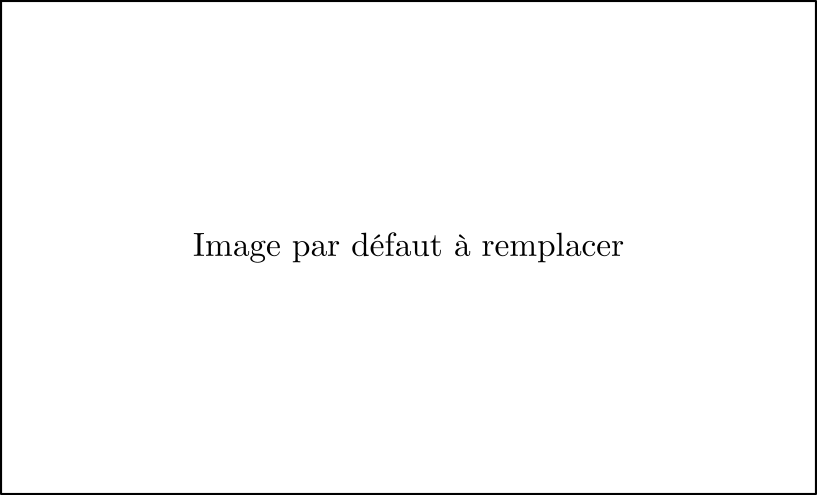
\includegraphics[width=0.5\linewidth]{defaut}
		\caption{Oscillogramme vérification procédure interruption}
	\end{figure}
	La fréquence du signal observé est de XXHz. 
	
	Cette partie a permis de soulever un problème lié à une programmation conjointe logiciel matériel et de proposer un solution, les interruptions. Le fonctionnement globale du système d'interruption des microcontrôleurs basés sur un Cortex-M a pu être détaillé. La configuration à travers un exemple concret utilisant le TC6 a finalement illustré ces explications. 
	
	
	
	\newpage
	\section{Implémentation fonction calcul gabarit}
	Cette partie présente la conception de la fonction calcul gabarit conformément au cahier des charges donné dans le sujet. Elle a pour fonction de déterminer la vitesse de rotation du moteur, comprise entre 0 et 5000 tr/min, en fonction du temps. Le gabarit se décompose en trois phases :
	\begin{itemize}
		\item accélération d'une durée de 128 ms
		\item vitesse constante d'une durée de 512 ms
		\item décélération d'une durée de 128 ms
	\end{itemize}
	La valeur du palier correspondant à la vitesse constante est un paramètre variable fournis par un bloc externe avec une précision de 10 tr/min. Pour simplifier le problème elle ne pourra être modifiée au cours d'un cycle. A ce niveau dans le projet les blocs externes ne sont pas encore développés. Pour facilité l'observation lors de tests le gabarit sera généré en boucle. Un état Repos doit être ajouté pour les délimiter, sa durée sera de 64 ms.
	\subsection{Conception fonctionnelle}
	L'étape de conception fonctionnelle a pour objectif de définir une solution en ne considérant que l'aspect fonctionnel et sans tenir compte des contraintes technologiques. Il est donc question de trouver une solution en mesure de générer \textbf{le gabarit constitué des quatre étapes : repos, accélération, constante et décélération.} Ainsi la description sous forme d'un automate à état finis s'impose par la séquentialité du problème. La traduction donne le résultat suivant :
	\begin{figure}[H]
		\centering
		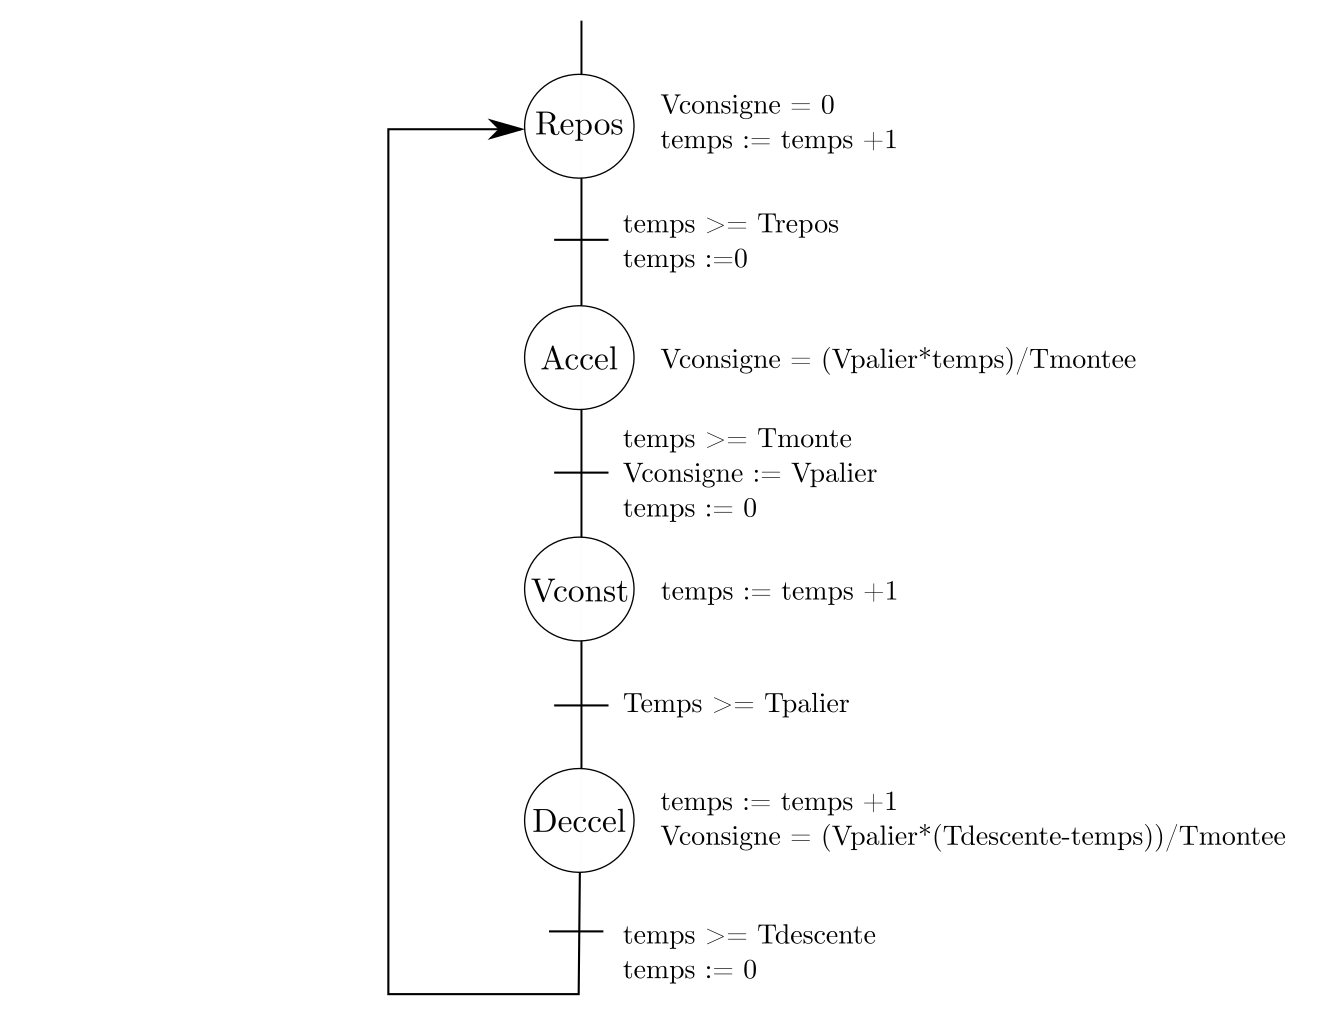
\includegraphics[width=0.76\linewidth]{calcul_gabarit_FSM}
		\caption{Description fonctionnelle calcul gabarit (FSM)}
		\label{fig:FSM}
	\end{figure}
	Cet automate est constitué des quatre états repos, accélération, constante et décélération et de leur transition respective. La variable \texttt{Vpalier} correspond au paramètre d'entrée de la fonction. Le résultat de l'exécution, placé dans \texttt{Vconsigne}, devra être communiqué au reste du système. 

	\newpage
	
	\subsection{Implémentation logicielle}
	La conception fonctionnelle précédente a permis de clarifié le problème. La première étape de la traduction en C est la déclaration des constantes. Elle se fait par l'instruction préprocesseur define ayant pour fonction de remplacer les instances suivantes de l'identifieur par la suite de lexèmes\footnote{Unité minimale de signification appartenant au lexique (Larousse)}. \cite{KRBook}
	\begin{lstlisting}[style=CStyle] 
	#define identifieur suite-de-lexemes \end{lstlisting}
	Ce procédé est utilisé pour définir les constantes utilisées ci-dessous. Le code C est le suivant :
	\begin{lstlisting}[style=CStyle] 
	#define TMontee 128
	#define TPalier 512
	#define TDescente 128
	#define TRepos 64\end{lstlisting}
	Les valeurs numériques proviennent directement du cahier des charges.
	
	Avant de traduire l'automate figure \ref{fig:FSM} il est important de définir précisément le type des variables utilisées.
	
	\begin{table}[H]
		\centering
		\begin{tabular}{|l|c|c|c|c|}
			\hline
			nom	 		& min	& max & type générique & type C \\ \hline
			temps		& 0		& 512	& entier & uint16\_t \\ \hline
			Vconsigne	& 0		& 5000	& entier & uint16\_t \\ \hline
			Vpalier		& 0		& 5000	& entier & uint16\_t \\
			\hline
		\end{tabular}
		\caption{Types des variables fonction calcul gabarit}
	\end{table}
	Le tableau ci dessus rassemble les informations permettant de choisir efficacement les types des variables. Elles sont toutes les trois entières, leur valeur minimum est supérieur à zéro et leur maximum compris entre 255 et 65535. Le type C correspondant est donc nécessairement uint16\_t. Il existe une autre variable implicite à l'implémentation d'un automate. C'est l'état courant \texttt{state} de type énumération. Il peut prendre pour valeur chacun des états repos, accélération, constante et décélération. Sa définition en langage C est la suivante :
	\begin{lstlisting}[style=CStyle] 
	enum state_t{Repos,Accel,Vconst,Decel};\end{lstlisting}
	Le type énumération correspond à un entier dont la taille peut contenir le nombre d'élément. Par défaut le premier élément vaut 0, et les suivants sont supérieures de 1 par rapport à la	valeur de la constante précédente. Il est possible d'affecter une valeur manuellement. Le guide des bonnes de pratiques de l'ANSSI\cite{ANSSI2021} indique par la règle 68 qu'il ne faut pas mélanger des constantes explicites et implicites dans une énumération pour éviter tout comportement indéterminé. Toute tentative d'affectation à une valeur non définie dans l'énumération provoquera une erreur à la compilation. Dans notre cas nous laisserons la définition à la charge du compilateur. Tel qu'est construit la machine état il est nécessaire de sauvegarder les valeurs des variables d'une exécution à l'autre. Il faudra donc ajouter le qualificateur \texttt{static}.\newline \indent
	Une fois les variables et constantes déclarées le corps de la fonction peut être implémenté. Il convient de convertir la machine état figure \ref{fig:FSM} en langage C. Cela se fait simplement autour d'un "\texttt{switch case}". Il est nécessaire de déclarer la variable \texttt{state} de type \texttt{state\_t}. Un cas par défaut a été ajouté à la description fonctionnelle pour couvrir les cas d'erreur. Lors d'une exécution normale la variable \texttt{state} ne peut prendre d'autres états que ceux déclarés dans l'énumération. Si toutefois, pour une raison inconnue, elle venait à prendre une autres valeurs, le programme se trouverait dans un état indéterminé et y resterait. Avec le cas défaut le programme peut se trouver dans un état non définit, mais il sera alors remis dans son état d'origine et l'exécution pourra continuée. L'implémentation en C est la suivante :
	
	
	\newpage

	
	\begin{lstlisting}[style=CStyle]
/* file : calcul_gabarit.c */

uint16_t calcul_gabarit (uint16_t VPalier){

	static uint16_t Temps = 0;
	static enum state_t state = Repos;
	static uint16_t Vconsigne = 0;
	
	switch (state)
	{
		case Repos :
			Vconsigne = 0;
			Temps ++;
			if(Temps >= 64){
			state = Accel;
			Temps = 0;
			}
			break;
	
		case Accel :
			if(Temps>=TMontee){
			state = Vconst;
			Temps = 0;
			Vconsigne = VPalier;
			}
			else{
			Temps ++;
			Vconsigne = (VPalier * Temps) / TMontee;
			}
			break;
	
		case Vconst :
			if (Temps>=TPalier){
			state = Decel;
			Temps = 0;
			}
			else{
			Temps ++;
			}
			break;
	
		case Decel:
			if(Temps >= TDescente){
			state = Repos;
			Temps = 0;
			Vconsigne = 0;
			}
			else{
			Temps ++;
			Vconsigne = (VPalier * (TDescente - Temps)) / TDescente;
			}
			break;
			
		default :
			state = Repos;
			Temps = 0;
			Vconsigne =0;
			break;
		}
		return Vconsigne;
	}
}	\end{lstlisting}

	\newpage
	\subsection{Test calcul gabarit et configuration DAC}
	La fonction calcul gabarit a été implémenté et doit donc être testée. Le résultat retourné est \texttt{Vconsigne}, dont la valeur analogique est comprise entre 0 et 5000. Pour visualiser son évolution dans le temps on peut s'appuyer sur un périphérique présent dans le SAMD21, le convertisseur numérique vers analogique (DAC : Digital Analog Converter). Ainsi il sera possible de visualiser le gabarit générer sous sa forme temporel tel qu'il a été décrit initialement dans le cahier des charges. Le DAC converti une valeur numérique en tension. Celui présent dans le microcontrôleur utilisé dispose d'une voix 10 bits sur 3,3V, soit une précision de 3,32mV. Sa représentation structurelle sous forme d'un diagramme bloc est la suivante :
	\begin{figure}[H]
		\centering
		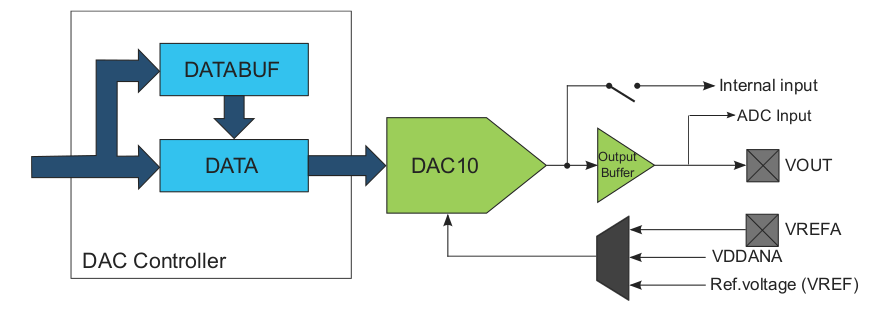
\includegraphics[width=0.75\linewidth]{DAC}
		\caption{Description diagramme bloc DAC}
	\end{figure}
	Les données à convertir transitent sur le bus APB BRIDGE C et doivent être dans le registre \texttt{DATA} ou \texttt{DATABUFER}. Ils correspondent respectivement à la valeur actuellement convertie et à la prochaine valeur convertie. Dans notre cas nous n'utiliserons que le registre \texttt{DATA}. Sa valeur est ensuite transmise à l'unité de conversion 10 bits dont la tension de référence, tension maximum, peut être sélectionnée parmi plusieurs sources. Le résultat sorte finalement sur une sortie interne, un buffer capable de débiter un courant plus important. Comme pour les autres périphériques un certain nombre de registres sont à disposition pour configurer ses nombreuses fonctionnalités.
	
	\paragraph{Configuration du registre CTRLA} ~~\\
	\begin{figure}[H]
		\centering
		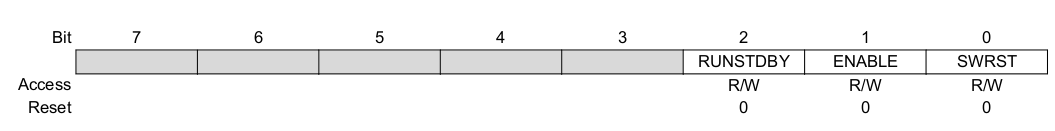
\includegraphics[width=12cm]{DAC_CTRLA}
		\caption{Description registre DAC CTRLA}
	\end{figure}
\begin{itemize}
	\item \textbf{SWRST} - Software Reset - Ce champ permet de remettre les registres du DAC dans leur état initial. Nous ne souhaitons pas faire cela, on écrira dans le registre \textbf{0 \textless \textless 0}\\
	\item \textbf{ENABLE} - Enable DAC Controller - Ce champ permet d'activer le Dac il faut donc écrire \textbf{1 \textless \textless 1} dans le registre.\\
	\item \textbf{RUNSTDBY} - Run in Standby - Ce champ permet d'activer ou de désactiver le buffer du DAC et mode veille. Dans notre cas cela a pet d'importance se bit peut être mis à 1 le laisser activé dans tous les cas : \textbf{1 \textless \textless 2}.
\end{itemize}

\paragraph{Configuration du registre CTRLB} ~~\\
\begin{figure}[H]
	\centering
	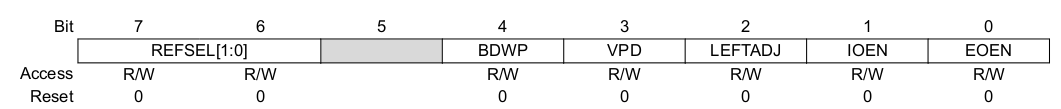
\includegraphics[width=12cm]{DAC_CTRLB}
	\caption{Description registre DAC CTRLB}
\end{figure}
\begin{itemize}
	\item \textbf{EOEN} - External Output Enable - Ce champ permet d'activer ou de désactiver la sortie du buffer. Nous ne souhaitons appliquer la tension sur le pin Vout,  on écrit dans le registre \textbf{1 \textless \textless 0}\\
	\item \textbf{IOEN} - Internal Output Enable - La sortie interne n'est pas utilisée on écrit \textbf{0 \textless \textless 1} dans le registre.\\
	\item \textbf{LEFTADJ} Left-Adjusted Data - La taille du registre \texttt{DATA} est de 16 bits mais seul les 10 premiers sont utilisés. Ce champs permet de sélectionner les bits en partant de la droite ou de la gauche. Dans notre cas les poids faibles sont à droite on choisira l'option d'alignement à droite. On écrit dans le registre \textbf{0 \textless \textless 2}\\
	\item \textbf{VPD} - Voltage Pump Disabled - Cette option permet d'économiser de l'énergie. Sa gestion et conservée comme automatique par l'écriture de \textbf{1 \textless \textless 3} dans le registre.\\
	\item \textbf{BDWP} - Bypass DATABUF Write Protection - Le registre DATABUF n'est pas utilisé, il n'est donc pas nécessaire de le protéger, on écrit \textbf{1 \textless \textless 4} dans le registre.\\
	\item \textbf{REFSEL[1:0]} - Reference Selection - Ce registre permet de sélectionner la source de tension de référence. Nous prendrons l'alimentation destinée aux circuits analogiques en écrivant  \textbf{0x1 \textless \textless 6} dans le registre.\\
\end{itemize}

\paragraph{Initialisation  du registre DATA} ~~\\
\begin{figure}[H]
	\centering
	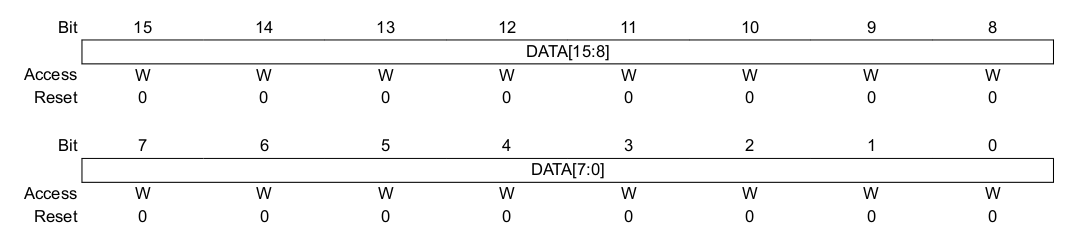
\includegraphics[width=12cm]{DATA}
	\caption{Description registre DAC CTRLB}
\end{figure}
Ce registre contient la valeur 10 bits à convertir dont l'alignement a été sélectionné avec le registre \texttt{LEFTADJ}. Pour tester la bonne configuration ce champ pourra être chargé à $1023/2$. Un tension de $3,3/3V$ devrait pouvoir être observée. 

\newpage

La configuration du DAC traduite en langage C donne le résultat suivant :
\begin{lstlisting}[style=CStyle]
void config_DAC(void){
	Dac *ptr_DAC = DAC ;
	
	ptr_DAC -> CTRLA.reg = 	DAC_CTRLA_RUNSTDBY 	|
                          DAC_CTRLA_ENABLE 		|
                          DAC_CTRLA_SWRST_NO ;
	
	ptr_DAC -> CTRLB.reg = 	DAC_CTRLB_REFSEL_AVCC	|
                          DAC_CTRLB_BDWP_NO			|
                          DAC_CTRLB_VPD_NO			|
                          DAC_CTRLB_LEFTADJ_NO  |
                          DAC_CTRLB_IOEN_NO 		|
                          DAC_CTRLB_EOEN ;
	/* Initialisation pour test */
	ptr_DAC -> DATA.reg = 1024/2;
	/* DATA.reg valeur 10bits max */
}
\end{lstlisting}
De nouveau l'utilisation des structures de l'ASF facilité grandement le travail. Cela améliore aussi la compréhension et donc la modification par un tiers.  


\newpage
\section{Implantation de la commande PWM et modélisation du moteur}
	Le cahier des charges requiert une commande de type PWM pour le moteur. Cette étape consiste à mettre en œuvre ce type de commande en utilisant un Timer. Le moteur sera quant à lui modélisé par un filtre passe-bas de constantes de temps 10ms. Éventuellement, ce filtre passe-bas pourra avoir une fonction d’atténuation, afin d’adapter le niveau de sortie du PWM à celui d'entrée du CAN. Le filtre sera alors réalisé par deux résistances et un condensateur. Selon la configuration du CAN qu’il sera bon d’étudier dans cette étape, il faudra trouver la structure de ce filtre ainsi que les valeurs des composants. 
	
\subsection{Génération du signal PWM}
	\subsubsection{Présentation la fonctionnement du TC en mode PWM}
	Il nous faut ici réaliser une commande de type PWM pour le moteur, représentative du gabarit mis en place. Le principe de la PWM est le suivant :  
	\begin{figure}[H]
	\centering
	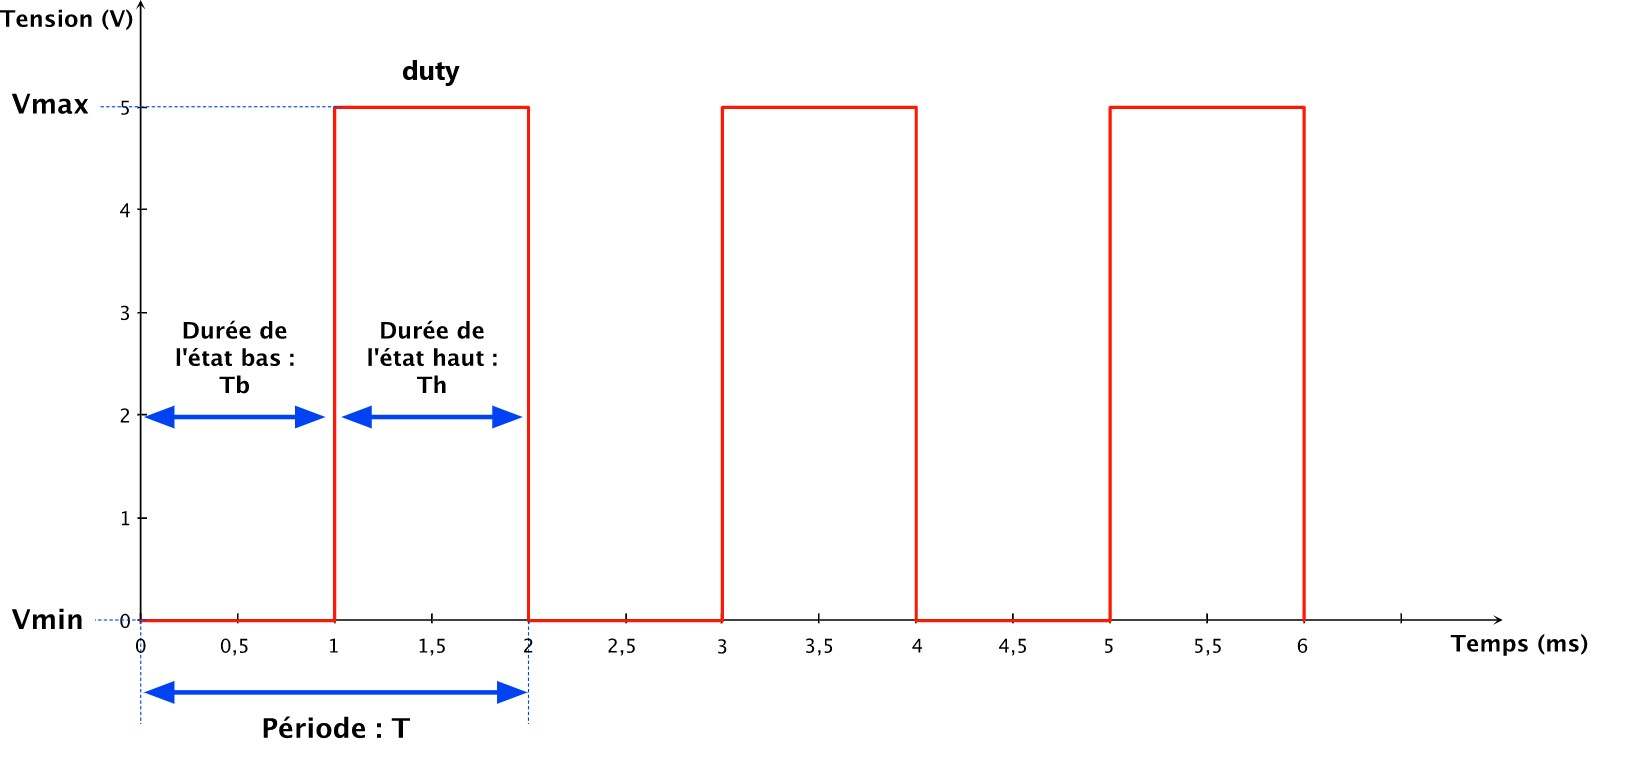
\includegraphics[width=10cm]{CaracPWM.jpg}
	\caption{Principe de la PWM}
    \end{figure}
	Le  signal  émis  est  rectangulaire  et  varie  entre  2  états  de  tension :  Umax  et  Umin (généralement  0V). La  tension  moyenne  de  ce signal,  notée  Umoy,  s’évalue de  la  façon suivante :  
	\begin{equation}
		U_{moy} = {\frac 1T}{\int_0^T {u(t)} \,{\rm d}t} = {\frac 1T}{[U_{max}*t]_0^{T_{h}}} = {U_{max}}{\frac {T_{h}}T}
	\end{equation}
	La tension moyenne ne dépend donc que du rapport cyclique entre $T_{h}$ et $T$. Si $T_{h}$ est nul, la tension moyenne est nulle. Si $T_{h}=T$, la tension moyenne est maximale. \\
	En se basant sur ce principe, le but est de transformer l’information de Vconsigne en une variation du rapport cyclique d’un signal envoyé au moteur. Si Vconsigne augmente, le rapport augmente et si Vconsigne atteint VpalierMax alors le rapport est maximal. Cette fonction est réalisable  grâce aux timers présent sur la carte. En effet il est possible de programmer un timer en mode MPWM (Match Pulse-Width Modulation). Le fonctionnement de ce mode est le suivant :
	\begin{figure}[H]
	\centering
	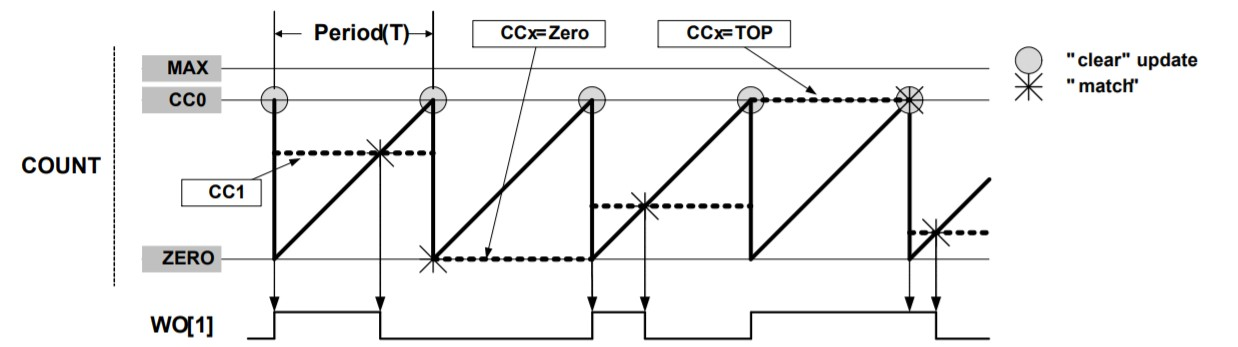
\includegraphics[width=0.9\linewidth]{mode_MPWM.jpg}
	\caption{Fonctionnement du mode MPWM}
    \end{figure}
    Ce mode permet de créer en sortie un signal de période définie par le rapport entre CC1 et CC0. Donc le rapport cyclique est contrôlable. Tant que COUNT a une valeur inférieur a CC1, WO[1] est à l'état haut puis il passe a l'état bas lorsque COUNT est entre CC1 est CC0. \\
    Le but de cette application étant d'avoir une fréquence de 10 kHz, il faut donc diviser l'horloge mère par 800 c'est à dire prendre un CC0 d'une valeur de 799. \\
    Le CC1 ne sera pas constant contrairement à CC0, il faudra l'actualiser à chaque fois que la vitesse imposée est changée soit toutes les microsecondes. La valeur de CC1 sera définie par la formule suivante:
    \begin{equation}
		CC1 = {\frac {Vconsigne*CC0} {VpalierMax}}={\frac {Vconsigne*799} {VpalierMax}}
	\end{equation}
    On sait que $0 \textless Vconsigne \textless {VpalierMax}$. CC1 évoluera donc entre 0 et CC0 ce qui permettra d'avoir un rapport cyclique entre 0 et 100\% comme souhaite.\\
    \subsubsection{Configuration et programmation}
    Au niveau, le timer TC7 sera utilisé. En effet celui-ci est déjà activé dans le registre GCLK car l’identifiant de TC7 est lié à celui de TC6 (voir partie 4.2). Il est donc préférable d’utiliser ce timer plutôt que d’en déclarer un nouveau. Les codes reprend en grande partie le principe de TC6 vu précédemment. \\
    La partie sur le registre GCLK n’a pas besoin d’être réécrite car TC6 et TC7 partageant le même identifiant, l’horloge est déclarée pour les 2 timers lors de l’initialisation de TC6. \\
    \paragraph{Configuration du Power Manager(PM)} ~~\\
    L’activation du timer TC7 auprès du Power Manager sans altérer les composants déjà présents. On ajout le code suivant dans le fonction config\_projet() qui est créé pour le TC6 au début:
    \begin{lstlisting}[style=CStyle]
void config_PM(void){
	    Pm *ptr_PM = PM;

	    ptr_PM -> APBCMASK.reg |=           PM_APBCMASK_TC7;
}
    \end{lstlisting}
    \paragraph{Configuration des ports d'E/S parallèles} ~~\\
    D’après la datasheet SAMD21, la sortie WO[1] du TC7 est disponible sur les pin PA21, PB01 et PB23. Pour des raisons pratiques vis-à-vis de la disposition des pins sur la carte, la pin PB01 est choisie. WO[1] est donc récupéré en sortie sur la pin 1 du port B en multiplexage E. On ajout le code suivant dans la méthode config\_PORT():
\begin{lstlisting}[style=CStyle]
void config_PORT(void){
	/* PWM */
	ptr_port -> Group[1].DIRSET.reg =  PORT_PB01;
	ptr_port -> Group[1].PMUX[1/2].reg = PORT_PMUX_PMUXO_E;
	ptr_port -> Group[1].PINCFG[1].reg = PORT_PINCFG_DRVSTR_NO |
	                                     PORT_PINCFG_PULLEN_NO |
	                                     PORT_PINCFG_INEN_NO |
	                                     PORT_PINCFG_PMUXEN;
}
\end{lstlisting}
    A noter que 1 est impair, il faut donc spécifier le multiplexage E dans la partie impaire du registre PMUX0. D’où l’utilisation de la constante PORT\_PMUX\_PMUXO\_E. 
    \paragraph{Configuration du périphérique Timer Counter 7} ~~\\
	Une nouvelle fonction \texttt{config\_PWM()} est créé dans le programme. \\
	La configuration du registre CTRLA du TC7, reprenant les mêmes éléments que pour TC6, sauf au niveau du mode sélectionné. Ici le mode est le MPWM et mis en place par la constante TC\_CTRLA\_WAVEGEN\_MPWM. 
\begin{lstlisting}[style=CStyle]
void config_PWM (void){
	Tc *ptr_TC = TC7 ;
	
	ptr_TC -> COUNT16.CTRLA.reg = TC_CTRLA_PRESCSYNC_PRESC |
	                              TC_CTRLA_NORUNSTDBY |
	                              TC_CTRLA_PRESCALER_DIV1 |
	                              TC_CTRLA_WAVEGEN_MPWM |
	                              TC_CTRLA_MODE_COUNT16 |
	                              TC_CTRLA_NOENABLE |
	                              TC_CTRLA_NOSWRST;
	//......
}
\end{lstlisting}~~\\
	La configuration des registres CTRLC et CTRLBCLR du TC7, reprenant la même logique que pour TC6, d’où la configuration similaire.
\begin{lstlisting}[style=CStyle]
    ptr_TC -> COUNT16.CTRLC.reg = TC_CTRLC_NOCPTEN0 |
                                  TC_CTRLC_NOCPTEN1 |
                                  TC_CTRLC_NOINVEN0 |
                                  TC_CTRLC_NOINVEN1;
	
    ptr_TC -> COUNT16.CTRLBCLR.reg = TC_CTRLBCLR_CMD_NONE |
                                     TC_CTRLBCLR_ONESHOT |
                                     TC_CTRLBCLR_NODIR;
\end{lstlisting}~~\\
	La configuration des 2 champs CC0 et CC1. CC1 est initialisé à 400 et variera par la suite. CC0 est affecté de la constante TC\_CC0\_Val, constante à la valeur 799 comme exprimé précédemment. 
\begin{lstlisting}[style=CStyle]
    ptr_TC -> COUNT16.CC[0].reg = TC_CC0_Val; // 10kHz
    ptr_TC -> COUNT16.CC[1].reg = 400; // duty 50%
\end{lstlisting}~~\\
    L’activation du timer TC7 en fin d’initialisation.
\begin{lstlisting}[style=CStyle]
    ptr_TC -> COUNT16.CTRLA.reg |= TC_CTRLA_ENABLE;
\end{lstlisting}~~\\
    Le timer TC7  est à présent  défini, il faut  maintenant  mettre  en place la  fonction permettant de faire évoluer le palier CC1 en fonction de $duty$ (Vconsigne). Cette fonction est la suivante :  
\begin{lstlisting}[style=CStyle]
void write_PWM (uint16_t duty){
	Tc *ptr_TC = TC7 ;
	
	ptr_TC -> COUNT16.CC[1].reg = (duty * TC_CC0_Val) / V_MAX;
}
\end{lstlisting}
    CC1 est défini sur [0 : TC\_TC0\_Val], c’est-à-dire [0 : 799]. V\_MAX est la constante de la valeur 5000.
\subsection{Dimensionnement du filtre modélisant le moteur}
	\subsubsection{Calculs pour un filtre passe bas}
	Pour ce projet, le moteur est représenté par une un filtre passe-bas ainsi qu’un étage d’atténuation (pour effectuer des ajustements sur les plages de tension) composés de résistances et de condensateurs. La structure utilisée est la suivante:	
	\begin{figure}[H]
	\centering
	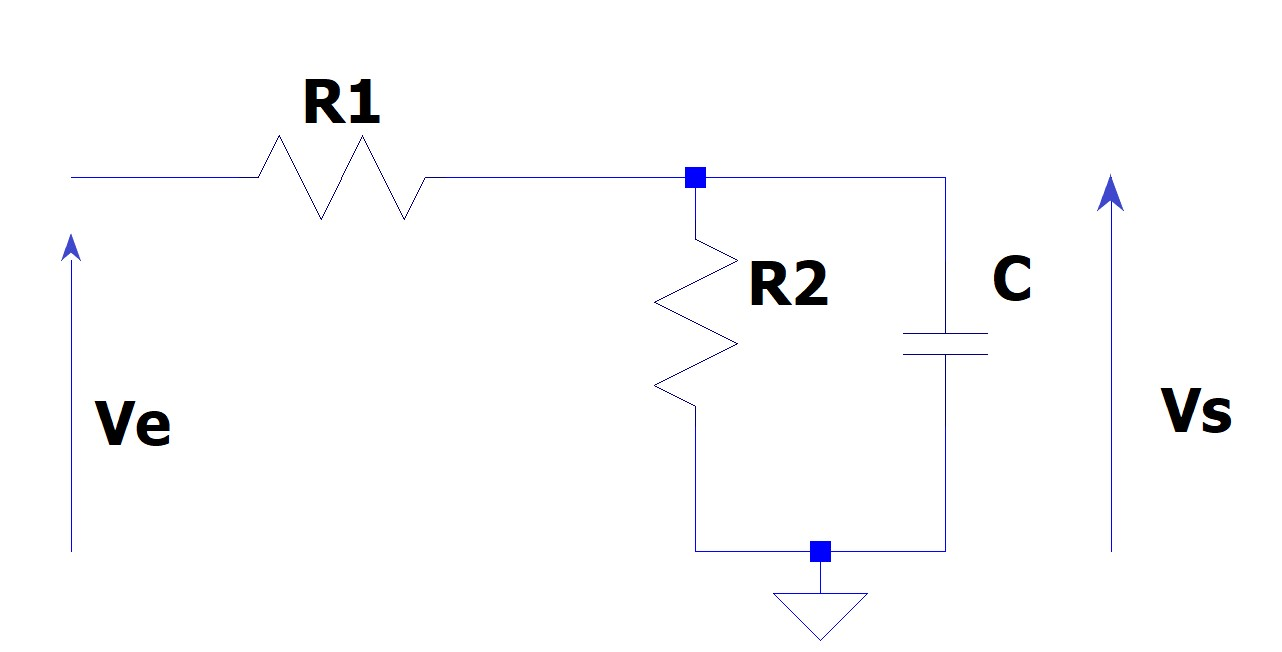
\includegraphics[width=0.6\linewidth]{filtre_RC.jpg}
	\caption{Schéma du filtre passe-bas}
    \end{figure}
    La fonction de transfert est déterminée par l’équation suivante:
    \begin{equation}
		H(p)={\frac {G}{1+\tau p}}
	\end{equation}
	Avec
	\begin{equation}
		G={\frac {V_s}{V_e}}={\frac {R_{2}} {R_{1}+R_{2}}}
	\end{equation}
	\begin{equation}
		\tau=(R_{1}//R_{2}) C={\frac {R_{1}R_{2}} {R_{1}+R_{2}}}C
	\end{equation}
	Il nous à présent dimensionner les composants. Le choix du filtre doit permettre d’avoir une tension de sortie égale à $\frac {3,3}{2}$V c’est-à-dire 1,65V. Pour cela, il faut travailler avec REFSEL à 0x2 pour avoir INTVCC1, c’est-à-dire $\frac 12$ de $V_{DDANA}$ mais tant que cela reste [valeur comparée]\textless2,7V.\\
	\begin{figure}[H]
	\centering
	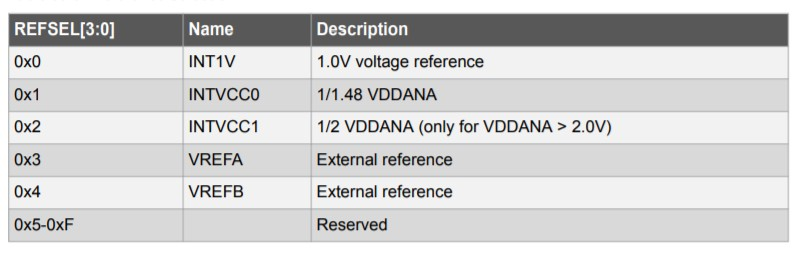
\includegraphics[width=0.8\linewidth]{Reference Selection_ADC.jpg}
	\caption{Tensions de références disponibles pour le CAN}
    \end{figure}
	Pour obtenir le signal désiré en sortie du filtre, il faut déterminer le gain. Celui-ci est $V_{DDANA}/2$ soit $G={\frac 12}$. De plus, la constante de temps de ce filtre est prise à 10 ms d’après le cahier des charges. Donc les composants reposent sur 2 conditions exprimées dans l’étape:
	\begin{itemize}
		\item {Constante de temps du filtre passe bas de 10ms }
		\item {Gain de 0,5}
	\end{itemize}
	Selon l'équation (8) et (9), on peut obtenir:
    \begin{equation}
		{\frac {R_{1}R_{2}} {R_{1}+R_{2}}}C = 10 ms
	\end{equation}
	\begin{equation}
		{\frac {R_{2}} {R_{1}+R_{2}}} = {\frac {1}{2}}
	\end{equation}
	D'après l'équation (11), on suppose que $R_{1}=R_{2}=R$. On peut obtenir alors 
	 \begin{equation}
		{\frac {R^2}{2R}} C={\frac {R}{2}}C = 10 ms
	\end{equation}
	Le choix de C étant limité dans les valeurs de composants existants, il est défini à 10 $\mu$F. Donc la valeur de R est 2,2 k$\Omega$. 
	\subsubsection{Test du filtre passe bas}
	Le circuit peut à présent être réalisé sur la planche à pain. Pour vérifier la constante de temps, nous utilisons l'oscilloscope pour observer la sortie du filtre. Le résultat est présenté dans la figure ci-dessous:
	\begin{figure}[H]
	\centering
	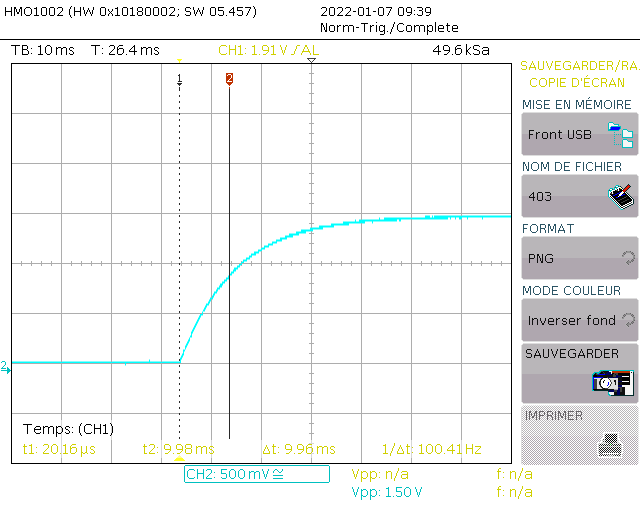
\includegraphics[width=0.8\linewidth]{test_filtre passe bas.PNG}
	\caption{Test de la sotie du filtre passe bas}
    \end{figure}
	D'après le résultat du test, la constante de temps est environ 10 ms qui vérifie le cahier des charges. Une fois le montage effectué, il suffit de relier les cartes ensemble ensuite de faire la simulation.
	
\subsection{Résultats de l’implantation}
    
  
	\bibliography{lib}{}
	\bibliographystyle{unsrt}
	
	\newpage
	
	\section{Annexe}
	
	\subsection{Programme C programmation TC6}
\begin{lstlisting}[style=CStyle]

#define GCLK_CLKCTRL_NOWRTLOCK        (0x0ul << GCLK_CLKCTRL_WRTLOCK_Pos)

#define GCLK_GENCTRL_NORUNSTDBY       (0x0ul << GCLK_GENCTRL_RUNSTDBY_Pos)
#define GCLK_GENCTRL_NODIVSEL         (0x0ul << GCLK_GENCTRL_DIVSEL_Pos)
#define GCLK_GENCTRL_NOOE             (0x0ul << GCLK_GENCTRL_OE_Pos)
#define GCLK_GENCTRL_NOOOV            (0x0ul << GCLK_GENCTRL_OOV_Pos)
#define GCLK_GENCTRL_NOIDC            (0x0ul << GCLK_GENCTRL_IDC_Pos)

#define TC_CTRLA_NORUNSTDBY           (0x0ul << TC_CTRLA_RUNSTDBY_Pos)
#define TC_CTRLA_NOENABLE             (0x0ul << TC_CTRLA_ENABLE_Pos)
#define TC_CTRLA_NOSWRST              (0x0ul << TC_CTRLA_SWRST_Pos)

#define TC_CTRLC_NOCPTEN0             (0 << TC_CTRLC_CPTEN0_Pos)
#define TC_CTRLC_NOCPTEN1             (0 << TC_CTRLC_CPTEN1_Pos)
#define TC_CTRLC_NOINVEN0             (0 << TC_CTRLC_INVEN0_Pos)
#define TC_CTRLC_NOINVEN1             (0 << TC_CTRLC_INVEN1_Pos)

#define TC_CTRLBCLR_NOONESHOT         (0x0ul << TC_CTRLBCLR_ONESHOT_Pos)

#define PORT_PINCFG_DRVSTR_NO          (0x0ul << PORT_PINCFG_DRVSTR_Pos)
#define PORT_PINCFG_PULLEN_NO          (0x0ul << PORT_PINCFG_PULLEN_Pos)
#define PORT_PINCFG_INEN_NO            (0x0ul << PORT_PINCFG_INEN_Pos)


Gclk *ptr_GCLK;
Pm *ptr_PM;
Port *ptr_port;
Tc *ptr_TC;

ptr_GCLK = GCLK;
ptr_GCLK->CLKCTRL.reg = GCLK_CLKCTRL_NOWRTLOCK |
								GCLK_CLKCTRL_CLKEN |
								GCLK_CLKCTRL_GEN_GCLK0 |
								GCLK_CLKCTRL_ID_TC6_TC7 ;

ptr_GCLK->GENCTRL.reg = GCLK_GENCTRL_NORUNSTDBY |
								GCLK_GENCTRL_NODIVSEL |
								GCLK_GENCTRL_NOOE |
								GCLK_GENCTRL_NOOOV |
								GCLK_GENCTRL_NOIDC |
								GCLK_GENCTRL_GENEN |
								GCLK_GENCTRL_SRC_OSC8M |
								GCLK_GENCTRL_ID(0);
									
	ptr_PM = PM;
	
	ptr_PM -> CPUSEL.reg = PM_CPUSEL_CPUDIV_DIV1;
	ptr_PM -> APBCSEL.reg = PM_APBCSEL_APBCDIV_DIV1;
	ptr_PM -> APBCMASK.reg |= PM_APBCMASK_TC6 | PM_APBCMASK_TC7 | PM_APBCMASK_DAC;
	
	ptr_port = PORT ;
	
	ptr_port -> Group[1].DIRSET.reg = PORT_PB02 | PORT_PB06 ; 
	ptr_port -> Group[1].PMUX[2/2].reg = PORT_PMUX_PMUXE_E;
	ptr_port -> Group[1].PINCFG[2].reg = PORT_PINCFG_DRVSTR_NO |
										PORT_PINCFG_PULLEN_NO |
										PORT_PINCFG_INEN_NO |
										PORT_PINCFG_PMUXEN;
	ptr_TC = TC6 ;
	
	ptr_TC -> COUNT16.CTRLA.reg = TC_CTRLA_PRESCSYNC_PRESC |
									TC_CTRLA_NORUNSTDBY |
									TC_CTRLA_PRESCALER_DIV1 |
									TC_CTRLA_WAVEGEN_MFRQ |
									TC_CTRLA_MODE_COUNT16 |
									TC_CTRLA_NOENABLE |
									TC_CTRLA_NOSWRST;
	ptr_TC -> COUNT16.CTRLC.reg = TC_CTRLC_NOCPTEN0 |
									TC_CTRLC_NOCPTEN1 |
									TC_CTRLC_NOINVEN0 |
									TC_CTRLC_NOINVEN1;
	ptr_TC -> COUNT16.CTRLBCLR.reg = TC_CTRLBCLR_CMD_NONE |
									TC_CTRLBCLR_ONESHOT |
									TC_CTRLBCLR_DIR;
	ptr_TC -> COUNT16.CC[0].reg = 7999;
	
	ptr_TC -> COUNT16.CTRLA.reg |= TC_CTRLA_ENABLE;	
	\end{lstlisting}
\end{document}

\begin{itemize}
	\renewcommand{\labelitemi}{--}
\end{itemize}